\documentclass{mathnote}
\usepackage{mathnote}

\begin{document}

% タイトルページの呼び出し
\tituloum
  {Analysis}
  {Namachan}
  {Mathematics Notes}
  {An introduction to limits, differentiation, and integration}
  {\today}

%\include{Preambulo/Capa}

\cleardoublepage
\pagenumbering{arabic}
\pagecolor{white}

% 目次
\localtableofcontents

\phantomsection
\part{数}

\begin{abstract}
この章では，解析学の議論の土台となる「数」に関する用語や概念を整理する．まず高校までに学んだ数の体系を振り返り，自然数から複素数へと数を拡張してきた動機を確認する．次に，実数の順序構造に注目し，最大元・最小元，上界・下界といった概念を定義する．そのうえで，最大元・最小元の一般化として上限・下限を導入し，その判定条件をいくつかの形で与える．これらの概念は，\partref{実数の連続性}で「実数の連続性」を述べるための言葉として不可欠なものである．

なお，解析学を学習するにあたって，日本の大学の講義においてはまず「数列の極限」を定義し直すことから始めることが多い．大学で学ぶ「実数列の収束」の定義（\partref{極限}）は次のようなものである：
  \begin{quotation}
  実数列 $(a_n)_{n \in \mathbb{N}}$ が $a \in \mathbb{R}$ に収束するとは，次が成り立つことである：

  任意の $\varepsilon > 0$ に対して，ある $n_0 \in \mathbb{N}$ が存在し，すべての $n \in \mathbb{N}$ に対して $n \geqq n_0$ ならば
  \[
    \abs{a_n - a} < \varepsilon
  \]
  が成立する．
  \end{quotation}
この定義は，いわゆる$\varepsilon$--$N$論法とよばれるものであり，高校で学んだ「数列がある値に限りなく近づく」という直感的な説明を厳密に表現したものである．
この定義を正確に理解するためにも，まずは「数」についていくつかの用語を定義することからはじめよう．
\end{abstract}

\phantomsection
\section{実数}

\phantomsection
\subsection{数の種類}

まず，高校で学んできた「数」を振り返ってみよう．

\begin{reviewbox}[数の集合]
  \small
  \begin{tabular}{@{}p{14\zw}@{\hspace{1.5\zw}}l@{}}
    自然数（natural numbers）&
    $\mathbb{N} = \{1,2,3,\ldots\}$\\[0.35\baselineskip]

    整数（integers）&
    $\mathbb{Z} = \{\ldots,-2,-1,0,1,2,\ldots\}$\\[0.35\baselineskip]

    有理数（rational numbers）&
    $\mathbb{Q} = \left\{ \frac{a}{b} \relmiddle| a \in \mathbb{Z},\ b \in \mathbb{N} \right\}$\\[0.35\baselineskip]

    実数（real numbers）&
    $\mathbb{R}$\\[0.35\baselineskip]

    複素数（complex numbers）&
    $\mathbb{C} = \{ a + bi \mid a,b \in \mathbb{R},\ i^2 = -1 \}$
  \end{tabular}
\end{reviewbox}

高校まではあまりなかった視点かもしれないが，ここで少し考察に付き合ってほしい．
$n,m\in\mathbb{N}$とすると $m+n\in\mathbb{N}$，$mn\in\mathbb{N}$である．大学で学ぶ言葉を使うと，このことは「$\mathbb{N}$は加法と乗法に関して閉じている」という\footnote{「閉じている」とは，ある集合に対して，その集合の要素同士で演算を行ったときに，結果もその集合の要素になることを指す．}．
しかし $n-m$ や $n\div m$ は $\mathbb{N}$ に属さない場合がある（たとえば $2-3$ や $2\div 3$）．

このことから，我々は自然数を拡張して整数，さらに有理数を導入した．実際，任意の $a,b\in\mathbb{Q}$ に対して
$ a + b \in \mathbb{Q}$，$ a - b \in \mathbb{Q}$，$ a \cdot b \in \mathbb{Q}$，$ a \div b \in \mathbb{Q}\ (b \ne 0)$
が成り立つ．このように，有理数は加法，減法，乗法，除法に関して閉じている．

しかし，$\mathbb{Q}$にも属さない数がある．たとえば $\sqrt{2}$ は有理数に属さない．さらに数列
\[
 a_n = \left( 1+\frac{1}{n} \right)^n
\]
を考えると，各 $n \in \mathbb{N}$ で $a_n\in\mathbb{Q}$ であるにもかかわらず，
\[
\lim_{n \to \infty} \left(1+\frac{1}{n}\right)^n = e \in \mathbb{R} \setminus \mathbb{Q}
\]
となり，極限として無理数が現れる．つまり，有理数列の極限が無理数になる場合もあるのである．

これらをふまえ，実数体 $\mathbb{R}$ を考えるにあたって，空でない部分集合
$A\subset\mathbb{R}$ が上に有界であるならば，$A$の上限 $\sup A$ が
$\mathbb{R}$ に存在することを，\textbf{実数の連続性の公理}として認めることにする%
\footnote{同様に，空でない部分集合 $A\subset\mathbb{R}$ が下に有界であるならば，$A$の下限 $\inf A$ も $\mathbb{R}$ に存在する．}．

さらに我々は $i=\sqrt{-1}$ を満たす数 $i$ を導入し，複素数体 $\mathbb{C}$ を構成する．
このようにして，自然数 $\mathbb{N}$，整数 $\mathbb{Z}$，有理数 $\mathbb{Q}$，実数 $\mathbb{R}$，複素数 $\mathbb{C}$ という数の体系が構築される．

これらを踏まえた上で，厳密に「数」に関する議論を進めていきたいが，そのためにはいくつかの用語を定義する必要がある．
そこでまずは「慣れ親しんだ集合」として，$\mathbb{R}$ の部分集合 $A$ を中心に議論を進めていこう．

\phantomsection
\subsection{実数の順序構造}

\begin{prop}{実数の稠密性}{real_dense}
任意の$a,b \in \mathbb{R}$に対して，$a < b$ ならば
\[
a < c < b
\]
を満たす $c \in \mathbb{R}$ が存在する．
\end{prop}

\begin{tleftbar}
\begin{proof}
$c = (a+b)/2$ とおけば，これは $a < c < b$ を満たす．
\end{proof}
\end{tleftbar}

命題\prref{real_dense}の証明では，やや天下り的に
「$c = (a+b)/2$ とおけばよい」と書いた．
我々は，理由をいっさい述べることなくこのような数をとることにした．
しかし，このように$c$を選ぶと都合がいいことは，数直線上で $a$ と $b$ のちょうど真ん中にある数を選んでいると考えれば自ずと理解できる．

もちろん，$c$ の選び方は一通りではない．
たとえば，$a$と$b$の対数平均を考えて，
\[
  c = \frac{b-a}{\log b - \log a}
\]
とおいても，$a < c < b$ が成り立つ．
また，証明において重要なのは，条件を満たす $c$ が少なくとも1つ存在することを示すことであり，
その $c$ をどのように発見したかまで説明する必要はない．

\begin{prop}{任意の正数より小さい非負実数}{nonnegative_less_than_all_positive}
  $a \geqq 0$ とする．
  任意の $\varepsilon > 0$ に対して $a < \varepsilon$ が成り立つならば，
  $a = 0$ である．
\end{prop}

\begin{tleftbar}
\begin{proof}
背理法で示す．
$a \neq 0$ と仮定する．
$a \geqq 0$ であるから，このとき $a > 0$ である．

命題\prref{real_dense}より，$0 < \varepsilon < a$ を満たす
$\varepsilon \in \mathbb{R}$ が存在する．
特に $\varepsilon > 0$ であるが，仮定より $a < \varepsilon$ でなければならない．
これは $\varepsilon < a$ に矛盾する．

したがって，$a = 0$ である．これが証明すべきことであった．
\end{proof}
\end{tleftbar}

\begin{remark}[「任意の$\varepsilon>0$」の読み方]
  ここで，「任意の $\varepsilon>0$ に対して $a<\varepsilon$ が成り立つ」とは，ある特定の $\varepsilon$ に対してのみ成り立つという意味ではなく，どれほど小さい正数 $\varepsilon$ をとっても $a<\varepsilon$ が成り立つという意味である．
  たとえば，$a=1$ として $\varepsilon=2$ をとれば確かに $a<\varepsilon$ となるが，これは仮定を満たすことを意味しない．実際，$\varepsilon=1/2$ とすれば $a<\varepsilon$ は成り立たない．
  したがって，$a>0$ である限り，$a$ より小さい正数 $\varepsilon$ をとることで必ず仮定に反する．
\end{remark}

ここまででは，実数どうしの大小関係について考えてきた．
次に，ある集合の中で「最も大きい元」や「最も小さい元」を考える．
このような元を，それぞれ最大元・最小元という．

\begin{definition}{最大元・最小元}{最大元・最小元}
  \index{さいだいげん@最大元}\index{さいしょうげん@最小元}
  $A \subset \mathbb{R}$とする．

  $m \in \mathbb{R}$が
  \[
    \begin{cases}
      \textup{(1)}\ m \in A,\\
      \textup{(2)}\ \forall x \in A,\ x \leqq m
    \end{cases}
  \]
  を満たすとき，$m$を$A$の\emph{最大元}といい，
  \[
    m = \max A
  \]
  とかく．

  また，$m \in \mathbb{R}$が
  \[
    \begin{cases}
      \textup{(1)}\ m \in A,\\
      \textup{(2)}\ \forall x \in A,\ m \leqq x
    \end{cases}
  \]
  を満たすとき，$m$を$A$の\emph{最小元}といい，
  \[
    m = \min A
  \]
  とかく．
\end{definition}

\begin{remark}[最大元と最大値]
  「最大元」と似た言葉に「最大値」がある．
  これらは密接に関係しているが，何について述べているかが異なる．
  最大元は，集合そのものに対して定めた言葉である．
  一方，関数$f \colon D \to \mathbb{R}$について「$f$の最大値」というときは，
  $f$の値全体の集合
  \[
    f(D) = \{f(x) \mid x \in D\}
  \]
  の最大元のことをいう．
  すなわち
  \[
    \max_{x \in D} f(x) \coloneqq \max f(D)
  \]
  であり，関数の最大値は，その値全体の集合の最大元として捉えることができる．
  この意味で，本書では，関数については最大値，集合については最大元という語を用いる\footnote{%
    ただし，$\max A$，$\min A$を「$A$の最大値」「$A$の最小値」とよぶことも
    広く行われており，これらが誤りというわけではない．%
  }．
  最小値と最小元についても同様である．

  なお，$\max_{x \in D} f(x)$は最大値であって，$D$の元ではない．
  これに対し，$f(a) = \max f(D)$を満たす$a \in D$を，
  $f$が最大値をとる点という．
  最大値は存在すればただ一つに定まるのに対し，
  最大値をとる点は複数存在しうる．
  たとえば$f(x) = x^{2}$，$D = [-1,1]$のとき，
  最大値は$1$であるが，これをとる点は$x = 1$と$x = -1$の2つである．
\end{remark}

\begin{figure}[htbp]
  \centering
  \begin{tikzpicture}[scale=1.0, >=stealth]

    % ==================================================
    % A = (0,1]
    % ==================================================

    % 数直線
    \draw[->, thick, black] (-0.5,1.3) -- (5.2,1.3);

    % 集合 A
    \draw[line width=2pt, magenta] (1,1.3) -- (4,1.3);

    % 端点
    % 0: A に含まれない
    \draw[thick, magenta, fill=white] (1,1.3) circle (2.5pt);
    % 1: A に含まれる
    \filldraw[magenta] (4,1.3) circle (2.5pt);

    % 目盛り
    \node[below] at (1,1.15) {$0$};
    \node[below] at (4,1.15) {$1$};

    % 集合名（線と重ならないように左上へ）
    \node[above left] at (-0.25,1.3) {$A$};

    % 最大元
    \node[above, magenta] at (4,1.45) {最大元};

    % 補足
    \node[right, align=left] at (5.4,1.3)
      {$A=(0,1]$\\最小元は存在しない};

    % ==================================================
    % B = [0,1)
    % ==================================================

    % 数直線
    \draw[->, thick, black] (-0.5,-0.2) -- (5.2,-0.2);

    % 集合 B
    \draw[line width=2pt, magenta] (1,-0.2) -- (4,-0.2);

    % 端点
    % 0: B に含まれる
    \filldraw[magenta] (1,-0.2) circle (2.5pt);
    % 1: B に含まれない
    \draw[thick, magenta, fill=white] (4,-0.2) circle (2.5pt);

    % 目盛り
    \node[below] at (1,-0.35) {$0$};
    \node[below] at (4,-0.35) {$1$};

    % 集合名（線と重ならないように左上へ）
    \node[above left] at (-0.25,-0.2) {$B$};

    % 最小元
    \node[above, magenta] at (1,-0.05) {最小元};

    % 補足
    \node[right, align=left] at (5.4,-0.2)
      {$B=[0,1)$\\最大元は存在しない};

  \end{tikzpicture}
  \caption{最大元・最小元のイメージ}
\end{figure}

最大元・最小元は，単に集合の「端」にある数ではなく，その集合自身に属していなければならない．
したがって，集合に上端や下端が見えていても，その点が集合に含まれていなければ最大元・最小元は存在しない．

\begin{example}{最大元・最小元の例}{最大元・最小元の例}
    集合$A=\{x \mid x \in \mathbb{R},0<x \leqq 1\}$に対して，$\max A=1$，$\min A$は存在しない．
    集合$B=\{x \mid x \in \mathbb{R},0 \leqq x <1\}$に対して，$\min B=0$，$\max B$は存在しない．
\end{example}

\begin{prop}{最大元・最小元の一意性}{max_min_uniqueness}
    任意の集合$A$に対し，その最大元・最小元は存在するとすればただひとつである．
\end{prop}

\begin{tleftbar}
  \begin{proof}
    $m, m'$がともに集合$A$の最大元であると仮定する．
    最大元の定義より，
    \[
      m = \max A
      \quad\Longleftrightarrow\quad
      \begin{cases}
        \textup{(1)}\ m \in A,\\
        \textup{(2)}\ \forall x \in A,\ x \leqq m
      \end{cases}
    \]
    であり，同様に
    \[
      m' = \max A
      \quad\Longleftrightarrow\quad
      \begin{cases}
        \textup{(1)}\ m' \in A,\\
        \textup{(2)}\ \forall x \in A,\ x \leqq m'
      \end{cases}
    \]
    である．

    $m$は$A$の最大元であり，$m' \in A$であるから，
    \[
      m' \leqq m
    \]
    が成り立つ．また，$m'$は$A$の最大元であり，$m \in A$であるから，
    \[
      m \leqq m'
    \]
    が成り立つ．したがって，$m = m'$である．

    同様にして，最小元についても一意性が示される．これが証明すべきことであった．
  \end{proof}
\end{tleftbar}

\begin{remark}[一意性と記号の正当化]
  ところで，なぜわざわざ一意性を確認しなければならないのだろうか．
  それは，我々が\deref{最大元・最小元}において $m = \max A$ という「記号」を導入したからである．

  一般に，数学において記号を定めるときは，その記号が指し示す対象がただひとつに定まっていなければならない．
  たとえば，空集合を表す記号 $\varnothing$ は，「要素をもたない集合はただひとつしかない」という事実に支えられて初めて意味をもつ．
  また，正則行列 $A$ の逆行列を $A^{-1}$ とかくのも，「$AB = BA = E$ を満たす行列 $B$ は存在すればただひとつである」ことが証明されているからこそ許される記法である．
  もし条件を満たす対象が複数ありうるならば，記号がそのうちのどれを指しているのかが定まらず，たとえば $\max A = 1$ のような等式は意味をなさなくなってしまう．
  \prref{max_min_uniqueness}は，記号 $\max A$，$\min A$ の使用を正当化するための命題なのである．

  別の見方をすれば，$\max$ は「集合 $A$ を入力すると実数 $\max A$ を返す対応」，すなわち一種の写像とみなすこともできる%
  \footnote{ただし，最大元が存在しない集合には値を定めないので，正確には「最大元をもつ集合全体」を定義域とする写像である．}．
  写像とは，入力ひとつに対して出力を\emph{ただひとつ}定める対応のことであった．
  したがって，$\max$ をこのような写像として扱うためにも，最大元の一意性が保証されていなければならない．
  最小元 $\min$ についても同様である．
\end{remark}

ただ，最大元および最小元は，$\mathbb{R}$の部分集合すべてに存在するとは限らない．そこで，$[0,1)$や$(0,1]$のような最大元（最小元）のない集合にも，似た概念を与えたい．「最大元」および「最小元」に似た概念として「上限」と「下限」を定義しよう．そのために，まず上界・下界を定義する．

\begin{definition}{上界・下界・有界}{上界・下界・有界}
  \index{じょうかい@上界}\index{かかい@下界}\index{ゆうかい@有界}
  $A \subset \mathbb{R}$とする．

  $a \in \mathbb{R}$が
  \[
    \forall x \in A,\ x \leqq a
  \]
  を満たすとき，$a$を$A$の\emph{上界}という．
  また，$A$の上界全体の集合を$U(A)$とかく．すなわち，
  \[
    U(A) = \{ a \in \mathbb{R} \mid \forall x \in A,\ x \leqq a \}
  \]
  である．

  また，$a \in \mathbb{R}$が
  \[
    \forall x \in A,\ a \leqq x
  \]
  を満たすとき，$a$を$A$の\emph{下界}という．
  また，$A$の下界全体の集合を$L(A)$とかく．すなわち，
  \[
    L(A) = \{ a \in \mathbb{R} \mid \forall x \in A,\ a \leqq x \}
  \]
  である．

  そして，$A$が上にも下にも有界であるとき，$A$は\emph{有界}であるという．
\end{definition}

\deref{上界・下界・有界}は難解に思えるかもしれない．言わんとしていることは「$U(A)$は，$A$の中のどの要素よりも大きいかもしくは等しい数全体の集合」ということである．

具体例で説明しよう．

\begin{example}{上界・下界の例}{上界・下界の例}
  集合
  \[
    A = \{ x \in \mathbb{R} \mid 0 < x < 1 \}
  \]
  について，
  \[
    U(A) = [1,\infty),
    \quad
    L(A) = (-\infty,0]
  \]
  である．

  そして，集合$A$は有界である．
\end{example}

\begin{prop}{有界であるための必要十分条件}{boundedness_characterization}
  $A \subset \mathbb{R}$とする．

  \[
    A\ \text{が上に有界}
    \quad\Longleftrightarrow\quad
    U(A) \neq \varnothing
  \]
  である．また，
  \[
    A\ \text{が下に有界}
    \quad\Longleftrightarrow\quad
    L(A) \neq \varnothing
  \]
  である．
\end{prop}

\begin{leftbar}
\begin{proof}
  まず，上に有界であることについて示す．

  $A$が上に有界であるとする．
  このとき，$A$の上界が存在するので，$U(A) \neq \varnothing$である．

  逆に，$U(A) \neq \varnothing$であるとする．
  このとき，ある$a \in U(A)$が存在する．
  $U(A)$の定義より，すべての$x \in A$に対して$x \leqq a$である．
  したがって，$a$は$A$の上界であるから，$A$は上に有界である．

  下に有界であることについても，同様に議論を進めると，
  \[
    A\ \text{が下に有界}
    \quad\Longleftrightarrow\quad
    L(A) \neq \varnothing
  \]
  が成り立つ．これが証明すべきことであった．
\end{proof}
\end{leftbar}

\begin{prop}{}{}
  $A$が有界であることは，$U(A) \neq \varnothing$かつ$L(A) \neq \varnothing$であるための必要十分条件である．
\end{prop}

\begin{leftbar}
\begin{proof}
  $A$が有界であるとする．
  このとき，\deref{上界・下界・有界}により$A$は上に有界であるから，\prref{boundedness_characterization}により$U(A) \neq \varnothing$である．

  また\deref{上界・下界・有界}により，$A$は下に有界であるから\prref{boundedness_characterization}により$L(A) \neq \varnothing$である．

  逆に，$U(A) \neq \varnothing$かつ$L(A) \neq \varnothing$であるとする．
  このとき，\prref{boundedness_characterization}により$A$は上に有界であり，下に有界である．
  したがって，$A$は有界である．
\end{proof}
\end{leftbar}

\begin{example}{有界な集合}{有界な集合}
  集合
  \[
    A = \{ x \in \mathbb{R} \mid x > 1 \}
  \]
  は下に有界であるが，上に有界ではない．

  一方，集合
  \[
    B = \{ x \in \mathbb{R} \mid 1 < x < 4 \}
  \]
  は上にも下にも有界である．したがって，$B$は有界である．
\end{example}

\begin{definition}{上限と下限}{sup_inf}
  $A$を$\mathbb{R}$の空でない部分集合とする．

  $A$が上に有界であるとき，
  \[
    \sup A = \min U(A)
  \]
  と定める．このとき，$\sup A$を$A$の\emph{最小上界}または\emph{上限}という．

  また，$A$が下に有界であるとき，
  \[
    \inf A = \max L(A)
  \]
  と定める．このとき，$\inf A$を$A$の\emph{最大下界}または\emph{下限}という．
\end{definition}

% --- TikZ による図解 ---
\begin{figure}[htbp]
  \centering
  \begin{tikzpicture}[scale=0.8, >=stealth]
    % ==================================================
    % 領域
    % ==================================================
    % 下界・上界の領域を薄いマゼンタで表示
    \fill[magenta!8] (-7,0) rectangle (-2,1);
    \fill[magenta!8] (2,0) rectangle (7,1);
    % 集合 A の領域
    \fill[black!7] (-2,0) rectangle (2,1);
    % ==================================================
    % 数直線
    % ==================================================
    \draw[->, thick, black]
      (-7.5,0) -- (7.5,0)
      node[right] {$\mathbb{R}$};
    % ==================================================
    % inf A, sup A
    % ==================================================
    % 下限
    \draw[magenta, thick]
      (-2,0) -- (-2,1.2)
      node[above] {$\inf A$};
    % 上限
    \draw[magenta, thick]
      (2,0) -- (2,1.2)
      node[above] {$\sup A$};
    % 境界点
    \filldraw[magenta] (-2,0) circle (2pt);
    \filldraw[magenta] ( 2,0) circle (2pt);
    % ==================================================
    % 上界・下界を表す上辺
    % ==================================================
    \draw[thick, black]
      (-7,1) -- (-2,1);
    \draw[thick, black]
      (2,1) -- (7,1);
    % ==================================================
    % ラベル
    % ==================================================
    % 集合 A
    \node at (0,0.5) {$A$};
    % 下界全体
    \node[magenta] at (-4.5,0.5)
      {$L(A)$（下界）};
    % 上界全体
    \node[magenta] at (4.5,0.5)
      {$U(A)$（上界）};
  \end{tikzpicture}
  \caption{上限・下限と上界・下界のイメージ}
\end{figure}

\begin{remark}[上限・下限の一意性]
  ここで，上限・下限の一意性について確認しておこう．
  \deref{sup_inf}によれば，$\sup A$ は上界集合 $U(A)$ の最小元として，$\inf A$ は下界集合 $L(A)$ の最大元として定義されている．
  そして，\prref{max_min_uniqueness}により，最大元・最小元は存在すればただひとつであった．
  したがって，$\sup A$ および $\inf A$ も存在すればただひとつである（上限・下限の一意性）．
  すなわち，上限・下限の一意性は，新たに証明し直すまでもなく，最大元・最小元の一意性から直ちに従う．
  これにより，記号 $\sup A$，$\inf A$ の使用もまた正当化されるのである．
\end{remark}

\begin{theorem}{上限・下限の判定条件}{characterization}
  $A$を$\mathbb{R}$の空でない部分集合とする．

  $A$が上に有界であるとき，$m \in \mathbb{R}$について
  \[
    m = \sup A
    \quad\Longleftrightarrow\quad
    \begin{cases}
      \textup{(1)}\ \forall x \in A,\ x \leqq m,\\
      \textup{(2)}\ \forall a < m,\ \exists x \in A,\ a < x
    \end{cases}
  \]
  が成り立つ．

  また，$A$が下に有界であるとき，$m \in \mathbb{R}$について
  \[
    m = \inf A
    \quad\Longleftrightarrow\quad
    \begin{cases}
      \textup{(1)}\ \forall x \in A,\ m \leqq x,\\
      \textup{(2)}\ \forall a > m,\ \exists x \in A,\ x < a
    \end{cases}
  \]
  が成り立つ．
\end{theorem}

\begin{tleftbar}
\begin{proof}
  まず，上限の場合を示す．$A$の上界全体の集合を$U(A)$とする．
  上限の定義より，
  \[
    m = \sup A
    \quad\Longleftrightarrow\quad
    m = \min U(A)
  \]
  である．

  さらに，最小元の定義より，
  \[
    m = \min U(A)
    \quad\Longleftrightarrow\quad
    \begin{cases}
      \textup{(1)}\ m \in U(A),\\
      \textup{(2)}\ \forall a \in U(A),\ m \leqq a
    \end{cases}
  \]
  である．ここで，(2)の対偶をとると，
  \[
    \forall a \in U(A),\ m \leqq a
    \quad\Longleftrightarrow\quad
    a < m\ \text{ならば}\ a \notin U(A)
  \]
  である．したがって，
  \[
    m = \sup A
    \quad\Longleftrightarrow\quad
    \begin{cases}
      \textup{(1)}\ m \in U(A),\\
      \textup{(2)}\ a < m\ \text{ならば}\ a \notin U(A)
    \end{cases}
  \]
  となる．

  最後に，上界の定義より，
  \[
    m \in U(A)
    \quad\Longleftrightarrow\quad
    \forall x \in A,\ x \leqq m
  \]
  であり，また
  \[
    a \notin U(A)
    \quad\Longleftrightarrow\quad
    \exists x \in A,\ a < x
  \]
  である．ゆえに，
  \[
    m = \sup A
    \quad\Longleftrightarrow\quad
    \begin{cases}
      \textup{(1)}\ \forall x \in A,\ x \leqq m,\\
      \textup{(2)}\ a < m\ \text{ならば}\ \exists x \in A,\ a < x
    \end{cases}
  \]
  が成り立つ．

  下限の場合も同様である．$A$の下界全体の集合を$L(A)$とすると，
  \[
    m = \inf A
    \quad\Longleftrightarrow\quad
    m = \max L(A)
  \]
  である．最大元の定義より，
  \[
    m = \max L(A)
    \quad\Longleftrightarrow\quad
    \begin{cases}
      \textup{(1)}\ m \in L(A),\\
      \textup{(2)}\ \forall a \in L(A),\ a \leqq m
    \end{cases}
  \]
  である．(2)の対偶をとると，
  \[
    \forall a \in L(A),\ a \leqq m
    \quad\Longleftrightarrow\quad
    m < a\ \text{ならば}\ a \notin L(A)
  \]
  である．

  ここで，下界の定義より，
  \[
    m \in L(A)
    \quad\Longleftrightarrow\quad
    \forall x \in A,\ m \leqq x
  \]
  であり，また
  \[
    a \notin L(A)
    \quad\Longleftrightarrow\quad
    \exists x \in A,\ x < a
  \]
  である．したがって，
  \[
    m = \inf A
    \quad\Longleftrightarrow\quad
    \begin{cases}
      \textup{(1)}\ \forall x \in A,\ m \leqq x,\\
      \textup{(2)}\ \forall a > m,\ \exists x \in A,\ x < a
    \end{cases}
  \]
  が成り立つ．これが証明すべきことであった．
\end{proof}
\end{tleftbar}

\begin{theorem}{$\varepsilon$を用いた特徴づけ}{epsilon_delta}
  $A$を$\mathbb{R}$の空でない部分集合とする．

  $A$が上に有界であるとき，$m \in \mathbb{R}$について
  \[
    m = \sup A
    \quad\Longleftrightarrow\quad
    \begin{cases}
      \textup{(1)}\ \forall x \in A,\ x \leqq m,\\
      \textup{(2)}\ \forall \varepsilon > 0,\ \exists a \in A,\ m - \varepsilon < a
    \end{cases}
  \]
  が成り立つ．

  また，$A$が下に有界であるとき，$m \in \mathbb{R}$について
  \[
    m = \inf A
    \quad\Longleftrightarrow\quad
    \begin{cases}
      \textup{(1)}\ \forall x \in A,\ m \leqq x,\\
      \textup{(2)}\ \forall \varepsilon > 0,\ \exists a \in A,\ a < m + \varepsilon
    \end{cases}
  \]
  が成り立つ．
\end{theorem}

\begin{example}{集合 $A=[0,1)$ の上限・下限}{sup_inf_ex}
集合 $A \coloneqq [0,1)$ の上限 $\sup A$ と下限 $\inf A$ を，本節で導入した3通りの視点から導く．

\medskip
\noindent\textbf{(1) 上界集合 $U(A)$・下界集合 $L(A)$ による定義（\deref{上界・下界・有界}，\deref{sup_inf}）に基づく導出}

\begin{description}[labelwidth=6\zw, leftmargin=6.5\zw]
    \item[上限 $\sup A$：]
    まず上界集合 $U(A)$ を特定する．任意の $a \in A$ に対して $a < 1$ であるから，$1$ は $A$ の上界である．よって $1 \in U(A)$ となる．
    次に $x < 1$ とすると，$a \coloneqq (x+1)/2$ とおけば $x < a < 1$ より $a \in A$ かつ $a > x$ となるため，$x$ は上界ではない．
    これより $U(A) = [1, \infty)$ であり，その最小元（定義 \deref{最大元・最小元}）が上限であるから，$\sup A = \min U(A) = 1$ を得る．

    \item[下限 $\inf A$：]
    同様に下界集合 $L(A)$ を特定する．任意の $a \in A$ に対して $a \geqq 0$ であるから，$0$ は $A$ の下界である．よって $0 \in L(A)$ となる．
    次に $y > 0$ とすると，$a \coloneqq y/2$ とおけば $0 \leqq a < y$ より $a \in A$ かつ $a < y$ となるため，$y$ は下界ではない．
    これより $L(A) = (-\infty, 0]$ であり，その最大元が下限であるから，$\inf A = \max L(A) = 0$ である．
\end{description}

\medskip
\noindent\textbf{(2) 「上限・下限の判定条件」（定理 \thref{characterization}）による証明}

\begin{description}[labelwidth=6\zw, leftmargin=6.5\zw]
    \item[上限 $\sup A$：] $m=1$ とおく．
    \begin{itemize}
        \item \textbf{上界の条件}：任意の $a \in A = [0, 1)$ に対して $a < 1 \leqq 1$ より成り立つ．
        \item \textbf{最小性}：$x < 1$ とすると，$a \coloneqq (x+1)/2$ は $x < a < 1$ を満たし，$a \in A$ かつ $x < a$ となる要素が存在する．
    \end{itemize}
    よって，定理 \thref{characterization} より $1 = \sup A$ である．

    \item[下限 $\inf A$：] $m=0$ とおく．
    \begin{itemize}
        \item \textbf{下界の条件}：任意の $a \in A = [0, 1)$ に対して $a \geqq 0$ より成り立つ．
        \item \textbf{最大性}：$x > 0$ とすると，$a \coloneqq x/2$ は $0 \leqq a < x$ を満たし，$a \in A$ かつ $x > a$ となる要素が存在する．
    \end{itemize}
    よって，定理 \thref{characterization} より $0 = \inf A$ である．
\end{description}

\medskip
\noindent\textbf{(3) 「$\varepsilon$ を用いた特徴づけ」（定理 \thref{epsilon_delta}）による証明}

\begin{description}[labelwidth=6\zw, leftmargin=6.5\zw]
    \item[上限 $\sup A$：] $m=1$ とおく．
    \begin{enumerate}
        \item 任意の $a \in A$ に対して $a \leqq 1$ である（上界の性質）．
        \item 任意の $\varepsilon > 0$ に対して，$a \in A$ を以下のように選ぶ：
        \[
            a \coloneqq \begin{cases} 1 - \dfrac{\varepsilon}{2} & (0 < \varepsilon \leqq 1) \\[6pt] 0 & (\varepsilon > 1) \end{cases}
        \]
        このとき $a \in [0, 1)$ であり，いずれの場合も $1 - \varepsilon < a$ が成り立つ．
    \end{enumerate}
    よって，定理 \thref{epsilon_delta} より $\sup A = 1$ である．

    \item[下限 $\inf A$：] $m=0$ とおく．
    \begin{enumerate}
        \setcounter{enumi}{2}
        \item 任意の $a \in A$ に対して $a \geqq 0$ である（下界の性質）．
        \item 任意の $\varepsilon > 0$ に対して，$a \coloneqq \min\{\varepsilon/2, 1/2\}$ とおけば，$a \in A$ かつ $a < 0 + \varepsilon$ が常に成り立つ．
    \end{enumerate}
    よって，定理 \thref{epsilon_delta} より $\inf A = 0$ である．
\end{description}

以上より，結論として
\[
\sup A = 1, \quad \inf A = 0
\]
を得る．どの視点から導いても同じ結論に到達することを確認してほしい．
\end{example}


\part{極限}

\begin{abstract}
解析学の学習において，高校で「数列の極限」を定義する際に用いられた「限りなく近づく」という表現は，厳密な議論を行う上では曖昧さを残すものである．
本章では，この曖昧な表現を論理的に厳格な形へと再定義した $\varepsilon$--$N$ 論法を導入し，実数列の収束と発散を定義する．
さらに，数列を自然数から実数への「写像」として捉え直し，「極限の一意性」を証明する ．
また，極限操作が順序関係を保存することや，未知の数列の収束を判定する強力な手法である「はさみうちの原理」について，具体例を丁寧に確認していく．
このような厳密な議論は，次章以降において「実数の連続性」を数学的に記述するために不可欠である．
\end{abstract}

\phantomsection
\section{実数列の極限} \index{きょくげん@極限}
\subsection{実数列の性質}
\label{sec:実数列の極限}

高校数学において，数列の極限は次のように定義されていたはずである．

\begin{quotation}
  数列 $(a_n)_{n \in \mathbb{N}}$ \footnote{高校数学では数列を $\{a_n\}$ と表記することが多いが，大学数学では $n$ が自然数であることを明示するために $(a_n)_{n \in \mathbb{N}}$ とかく．
  また，$\{a_n\}$ という記法は集合 $\{ a_n \mid n \in \mathbb{N} \}$ と混同しやすく，たとえば $a_n \coloneqq (-1)^n$ のとき，数列としては各項が振動するが，
  集合としては $\{ -1, 1 \}$ という2要素のみを持つ集合を指すことになる．} 
  において，番号 $n$ を限りなく大きくするとき，$a_n$ の値がある一定の値 $a$ に限りなく近づくならば，この数列は $a$ に\textbf{収束する}といい，
  \[
    \lim_{n \to \infty} a_n = a
  \]
  と記す．
\end{quotation}

しかし，この「限りなく大きくする」「限りなく近づく」といった表現は直感的ではあるものの，数学的に厳密な定義とは言い難い．何をもって「限りなく」とするのか，その基準が曖昧だからである．
こうした直感的な表現を排し，論理的に厳格な形で実数列\footnote{各項が実数である数列のこと．}の収束を再定義したものが，以下の $\varepsilon\text{--}N$ 論法である．

\begin{definition}{実数列の収束}{実数列の収束} \index{じっすうれつのしゅうそく@実数列の収束}
  実数列 $(a_n)_{n \in \mathbb{N}}$ が $a \in \mathbb{R}$ に収束するとは，次が成り立つことである：
  
  任意の $\varepsilon > 0$ に対して，ある $n_0 \in \mathbb{N}$ が存在し，すべての $n \in \mathbb{N}$ に対して $n \ge n_0$ ならば
  \[
    \abs*{a_n - a} < \varepsilon
  \]
  が成立する．
\end{definition}



この定義は，「いかに小さな誤差 $\varepsilon$ を指定したとしても，ある番号 $n_0$ を境に，それ以降のすべての項 $a_n$ が $a$ の $\varepsilon$ 近傍，すなわち開区間 $(a-\varepsilon, a+\varepsilon)$ に収まってしまう」ことを意味している．

\begin{definition}{実数列の発散}{実数列の発散} \index{じっすうれつのはっさん@実数列の発散}
  実数列 $(a_n)_{n \in \mathbb{N}}$ が収束しないとき，その数列は\textbf{発散する}という\footnote{$a_n \coloneqq (-1)^n$ のように特定の定数に近づかず，かつ無限大にも行かない「振動」も，数学的には発散に含まれる．}．
\end{definition}

\begin{definition}{実数列の $+\infty$ への発散}{}
  実数列 $(a_n)_{n \in \mathbb{N}}$ が $+\infty$ に発散するとは，任意の $M \in \mathbb{R}$ に対して，ある $n_0 \in \mathbb{N}$ が存在し，すべての $n \in \mathbb{N}$ に対して $n \ge n_0$ ならば
  \[
    a_n > M
  \]
  が成立することである\footnote{$-\infty$ への発散の定義については，不等号の向きに注意して各自で考えてみてほしい．}．
\end{definition}

\subsection{実数列と極限の性質}

ここで，実数列を集合論的な観点から再定義しておく．数列とは，各自然数に対して一つの実数を割り当てる規則に他ならない．

\begin{definition}{実数列}{実数列}
  写像 $a \colon \mathbb{N} \to \mathbb{R}$ を実数列と呼ぶ．自然数 $n \in \mathbb{N}$ による像 $a(n)$ を $a_n$ と書き，数列そのものを $(a_n)_{n \in \mathbb{N}}$ と表記する．
\end{definition}


\begin{prop}{実数列の極限の一意性}{実数列の極限の一意性}
  数列 $(a_n)_{n \in \mathbb{N}}$ が収束するとき，その収束先（極限値）はただ一つに限る．
\end{prop}

\begin{leftbar}
\begin{proof}
  $a \ne b$ なる $a, b \in \mathbb{R}$ がともに数列 $(a_n)_{n \in \mathbb{N}}$ の収束先であると仮定し，矛盾を導く．
  $\varepsilon \coloneqq \frac{\abs*{b-a}}{2}$ とおくと，$a \ne b$ より $\varepsilon > 0$ である．
  収束の定義より，ある $n_0, n_1 \in \mathbb{N}$ が存在して，すべての $n \in \mathbb{N}$ に対して次が成り立つ：
  \[
    n \ge n_0 \implies \abs{a_n - a} < \varepsilon, \quad n \ge n_1 \implies \abs{a_n - b} < \varepsilon
  \]
  ここで $n \ge \max\{n_0, n_1\}$ を満たす $n$ を任意にとると，三角不等式より
  \[
    \abs{b-a} = \abs{(b - a_n) + (a_n - a)} \le \abs{a_n - b} + \abs{a_n - a} < \varepsilon + \varepsilon = 2\varepsilon = \abs{b-a}
  \]
  となり，$\abs{b-a} < \abs{b-a}$ という矛盾が生じる．したがって，収束先はただ一つである．
\end{proof}
\end{leftbar}

\begin{prop}{収束列の有界性}{収束列の有界性}
  収束する実数列は有界である．
\end{prop}


\begin{tleftbar}
\begin{proof}
  実数列$(a_n)_{n \in \mathbb{N}}$が$a \in \mathbb{R}$に収束するとする．
  このとき，収束の定義より，$1>0$に対して，ある$n_0 \in \mathbb{N}$が存在して，
  \[
    n \geqq n_0
    \implies
    \abs{a_n-a}<1
  \]
  が成り立つ．したがって，$n \geqq n_0$ならば，
  \[
    \abs{a_n}
    \leqq \abs{a_n-a}+\abs{a}
    < 1+\abs{a}
  \]
  である．

  また，$\abs{a_1},\abs{a_2},\ldots,\abs{a_{n_0}}$は有限個の実数であるから，
  \[
    M_0=\max\{\abs{a_1},\abs{a_2},\ldots,\abs{a_{n_0}}\}
  \]
  とおくことができる．

  そこで，
  \[
    M=\max\{M_0,\ 1+\abs{a}\}
  \]
  とおく．このとき，$n<n_0$ならば$\abs{a_n}\leqq M_0\leqq M$であり，
  $n\geqq n_0$ならば$\abs{a_n}<1+\abs{a}\leqq M$である．

  よって，すべての$n\in\mathbb{N}$に対して
  \[
    \abs{a_n}\leqq M
  \]
  が成り立つ．したがって，実数列$(a_n)_{n \in \mathbb{N}}$は有界である．
\end{proof}
\end{tleftbar}

\begin{theorem}{極限の四則演算}{極限の四則演算}
  実数列$(a_n)$，$(b_n)$がそれぞれ$a,b \in \mathbb{R}$に収束するとする．
  このとき，
  \[
    \lim_{n\to\infty}(a_n+b_n)=a+b,
    \qquad
    \lim_{n\to\infty}(a_nb_n)=ab
  \]
  が成り立つ．

  さらに，$b\ne 0$であり，十分大きい$n$に対して$b_n\ne 0$であるとき，
  \[
    \lim_{n\to\infty}\frac{a_n}{b_n}=\frac{a}{b}
  \]
  が成り立つ．
\end{theorem}

\begin{tleftbar}
\begin{proof}
  まず，和について示す．任意の$\varepsilon>0$をとる．
  $a_n\to a$，$b_n\to b$であるから，ある$n_1,n_2\in\mathbb{N}$が存在して，
  \[
    n\geqq n_1
    \implies
    \abs{a_n-a}<\frac{\varepsilon}{2}
  \]
  かつ
  \[
    n\geqq n_2
    \implies
    \abs{b_n-b}<\frac{\varepsilon}{2}
  \]
  が成り立つ．そこで，
  \[
    n_0=\max\{n_1,n_2\}
  \]
  とおく．このとき，$n\geqq n_0$ならば，
  \[
    \abs{(a_n+b_n)-(a+b)}
    =\abs{(a_n-a)+(b_n-b)}
    \leqq \abs{a_n-a}+\abs{b_n-b}
    <\frac{\varepsilon}{2}+\frac{\varepsilon}{2}
    =\varepsilon
  \]
  である．したがって，$a_n+b_n\to a+b$である．

  次に，積について示す．収束する実数列は有界であるから，$(b_n)$は有界である．
  よって，ある$M>0$が存在して，すべての$n\in\mathbb{N}$に対して
  \[
    \abs{b_n}\leqq M
  \]
  が成り立つ．

  任意の$\varepsilon>0$をとる．$a_n\to a$，$b_n\to b$であるから，ある$n_1,n_2\in\mathbb{N}$が存在して，
  \[
    n\geqq n_1
    \implies
    \abs{a_n-a}<\frac{\varepsilon}{2M}
  \]
  かつ
  \[
    n\geqq n_2
    \implies
    \abs{b_n-b}<\frac{\varepsilon}{2(\abs{a}+1)}
  \]
  が成り立つ．ただし，$\abs{a}+1>0$である．

  そこで，
  \[
    n_0=\max\{n_1,n_2\}
  \]
  とおく．このとき，$n\geqq n_0$ならば，
  \begin{align*}
    \abs{a_nb_n-ab}
    &=\abs{a_nb_n-ab_n+ab_n-ab} \\
    &\leqq \abs{b_n}\abs{a_n-a}+\abs{a}\abs{b_n-b} \\
    &\leqq M\abs{a_n-a}+\abs{a}\abs{b_n-b} \\
    &< M\cdot\frac{\varepsilon}{2M}
      +\abs{a}\cdot\frac{\varepsilon}{2(\abs{a}+1)} \\
    &\leqq \frac{\varepsilon}{2}+\frac{\varepsilon}{2}
     =\varepsilon
  \end{align*}
  である．したがって，$a_nb_n\to ab$である．

  最後に，商について示す．$b\ne 0$とする．
  まず，$b_n\to b$であるから，$\varepsilon=\dfrac{\abs{b}}{2}$に対して，
  ある$n_1\in\mathbb{N}$が存在して，
  \[
    n\geqq n_1
    \implies
    \abs{b_n-b}<\frac{\abs{b}}{2}
  \]
  が成り立つ．このとき，$n\geqq n_1$ならば，
  \[
    \abs{b_n}
    \geqq \abs{b}-\abs{b_n-b}
    >\abs{b}-\frac{\abs{b}}{2}
    =\frac{\abs{b}}{2}
  \]
  である．したがって，十分大きい$n$に対して$b_n\ne 0$である．

  任意の$\varepsilon>0$をとる．$a_n\to a$，$b_n\to b$であるから，ある$n_2,n_3\in\mathbb{N}$が存在して，
  \[
    n\geqq n_2
    \implies
    \abs{a_n-a}<\frac{\abs{b}}{2}\cdot \frac{\varepsilon}{2}
  \]
  かつ
  \[
    n\geqq n_3
    \implies
    \abs{b_n-b}<\frac{\abs{b}^2}{2(\abs{a}+1)}\cdot \frac{\varepsilon}{2}
  \]
  が成り立つ．

  そこで，
  \[
    n_0=\max\{n_1,n_2,n_3\}
  \]
  とおく．このとき，$n\geqq n_0$ならば，
  \begin{align*}
    \abs*{\frac{a_n}{b_n}-\frac{a}{b}}
    &=\abs*{\frac{b(a_n-a)-a(b_n-b)}{bb_n}} \\
    &\leqq \frac{\abs*{b}\abs*{a_n-a}+\abs*{a}\abs*{b_n-b}}
                  {\abs*{b}\abs*{b_n}} \\
    &< \frac{\abs*{b}\abs*{a_n-a}+\abs*{a}\abs*{b_n-b}}
             {\abs*{b}\cdot \dfrac{\abs*{b}}{2}} \\
    &= \frac{2}{\abs*{b}}\abs*{a_n-a}
       +\frac{2\abs*{a}}{\abs*{b}^2}\abs*{b_n-b} \\
    &< \frac{2}{\abs*{b}}\cdot\frac{\abs*{b}}{2}\cdot\frac{\varepsilon}{2}
       +\frac{2\abs*{a}}{\abs*{b}^2}\cdot
        \frac{\abs*{b}^2}{2(\abs*{a}+1)}\cdot\frac{\varepsilon}{2} \\
    &\leqq \frac{\varepsilon}{2}+\frac{\varepsilon}{2}
     =\varepsilon
  \end{align*}
  である．したがって，
  \[
    \frac{a_n}{b_n}\to\frac{a}{b}
  \]
  が成り立つ．
\end{proof}
\end{tleftbar}

ここで，$(a_n)$と$(b_n)$がともに収束する場合に，上の定理が成り立つことに注意しよう．
たとえば，
\[
  a_n \coloneqq n,
  \qquad
  b_n \coloneqq -n
\]
とすると，数列$(a_n+b_n)$は$0$に収束するが，数列$(a_n)$と$(b_n)$はともに発散する．
このように，極限の四則演算は，収束する数列に対して適用されるものである．



次に，極限操作が順序関係を保存することを示す．

\begin{theorem}{極限の不等式}{極限の不等式}
  収束する実数列 $(a_n)_{n \in \mathbb{N}}, (b_n)_{n \in \mathbb{N}}$ について，その極限をそれぞれ $a, b$ とする．
  
  すべての $n \in \mathbb{N}$ に対して $a_n \le b_n$ が成り立つならば，
  \[
    a \le b
  \]
  である．
\end{theorem}

\begin{leftbar}
\begin{proof}
  背理法を用いる．$a > b$ と仮定し，$\varepsilon \coloneqq \frac{a-b}{2} > 0$ とおく．
  収束の定義より，ある $n_0 \in \mathbb{N}$ が存在して，$n \ge n_0$ ならば
  \[
    \abs{a_n - a} < \varepsilon \implies a - \varepsilon < a_n < a + \varepsilon
  \]
  \[
    \abs{b_n - b} < \varepsilon \implies b - \varepsilon < b_n < b + \varepsilon
  \]
  がともに成立する．このとき，$b + \varepsilon = b + \frac{a-b}{2} = \frac{a+b}{2}$ および $a - \varepsilon = a - \frac{a-b}{2} = \frac{a+b}{2}$ であるから，
  \[
    b_n < b + \varepsilon = a - \varepsilon < a_n
  \]
  となり，すべての $n$ で $a_n \le b_n$ とした仮定に矛盾する．ゆえに $a \le b$ である．
\end{proof}
\end{leftbar}

注意すべき点は，元の数列の間に厳密な不等号 $a_n < b_n$ が成り立っていても，極限において不等号が維持されるとは限らないことである．
例えば，$a_n \coloneqq 1 - \frac{1}{n}$ および $b_n \coloneqq 1 + \frac{1}{n}$ とすると，任意の $n \in \mathbb{N}$ において $a_n < b_n$ が成立するが，極限値はともに $1$ となり，$a = b$ が成立してしまう．このように，極限操作によって不等号の「ゆとり」が消滅し，等号が成立する可能性がある．

\begin{theorem}{はさみうちの原理}{} \index{はさみうちのげんり@はさみうちの原理}
  実数列 $(a_n)_{n \in \mathbb{N}}, (b_n)_{n \in \mathbb{N}}$ がともに $a \in \mathbb{R}$ に収束するとする：
  \[
    \lim_{n \to \infty} a_n = a, \quad \lim_{n \to \infty} b_n = a
  \]
  このとき，別の数列 $(c_n)_{n \in \mathbb{N}}$ について，ある番号以上のすべての $n \in \mathbb{N}$ に対して
  \[
    a_n \le c_n \le b_n
  \]
  が成り立つならば，数列 $(c_n)_{n \in \mathbb{N}}$ もまた $a$ に収束する．すなわち，$(c_n) \in \mathcal{C}$ であり\footnote{ここでの $\mathcal{C}$ は，収束する実数列全体の集合を表す}，$\lim_{n \to \infty} c_n = a$ が成立する．
\end{theorem}



\begin{leftbar}
\begin{proof}
  任意の $\varepsilon > 0$ をとる．
  仮定より $\lim_{n \to \infty} a_n = a$ および $\lim_{n \to \infty} b_n = a$ であるから，この $\varepsilon$ に対してある $n_1, n_2 \in \mathbb{N}$ が存在し，次を満たす：
  \begin{align}
    n \ge n_1 &\implies a - \varepsilon < a_n < a + \varepsilon \\
    n \ge n_2 &\implies a - \varepsilon < b_n < a + \varepsilon
  \end{align}
  ここで $n_0 \coloneqq \max \{ n_1, n_2 \}$ と定めると，$n \ge n_0$ においては上の 2 つの不等式が同時に成立する．
  さらに，仮定 $a_n \le c_n \le b_n$ を合わせると， $n \ge n_0$ において
  \[
    a - \varepsilon < a_n \le c_n \le b_n < a + \varepsilon
  \in \]
  が成り立つ．したがって，$n \ge n_0$ ならば常に
  \[
    a - \varepsilon < c_n < a + \varepsilon \iff \abs{c_n - a} < \varepsilon
  \]
  が成立する．これは，数列 $(c_n)_{n \in \mathbb{N}}$ が $a$ に収束することの定義そのものである．
\end{proof}
\end{leftbar}

この原理の特筆すべき点は，数列 $(c_n)$ 自体の収束性をあらかじめ仮定する必要がないことにある．
上下から同じ値に収束する数列で「挟む」ことができれば，未知の数列 $(c_n)$ の収束先も同じ値であると結論づけることができる．このため，はさみうちの原理は数列の収束を判定する際の強力なツールとなる．

\begin{example}{はさみうちの原理（三角関数の例）}{はさみうちの原理（三角関数の例）}
	\[
	a_n \coloneqq \frac{\sin (\pi )}{n}
	\]
	とする．このとき， 
	\[
	- 1 \leqq \sin (\pi ) \leqq 1
	\]
	であるから，
	\[
	-\frac{1}{n} \leqq a_n \leqq \frac{1}{n}
	\]
	となり，$\lim_{n \to \infty} (-1/n)=0$，$\lim_{n \to \infty} 1/n =0$であるから，はさみうちの原理により，
	\[
	\lim_{n \to \infty} a_n =0.
	\]
\end{example}

\begin{example}{はさみうちの原理（ガウス記号の例）}{はさみうちの原理_ガウス}
  \[
    a_n \coloneqq \frac{\bigl[ \sqrt{n} \bigr]}{n}
  \]
  とする．このとき，任意の実数 $x$ に対して
  \[
    [x] \le x < [x] + 1
  \]
  が成り立つから，$x=\sqrt{n}$ とおくと
  \[
    \sqrt{n}-1 < \bigl[\sqrt{n}\bigr] \le \sqrt{n}
  \]
  となる．よって両辺を $n$ で割れば
  \[
    \frac{\sqrt{n}-1}{n} < a_n \le \frac{\sqrt{n}}{n}
  \]
  を得る．ここで
  \[
    \lim_{n\to\infty}\frac{\sqrt{n}-1}{n}
    = \lim_{n\to\infty}\left(\frac{1}{\sqrt{n}}-\frac{1}{n}\right)=0,
    \quad
    \lim_{n\to\infty}\frac{\sqrt{n}}{n}
    =\lim_{n\to\infty}\frac{1}{\sqrt{n}}=0
  \]
  であるから，はさみうちの原理により
  \[
    \lim_{n\to\infty} a_n = 0.
  \]
\end{example}


\part{実数の連続性}

\begin{abstract}
前章では，$\varepsilon$--$N$論法を用いることで，（実）数列の収束を厳密に定義した．
しかし，有理数列 $a_n = (1+1/n)^n$ が有理数の範囲に極限を持たないように，
「数列の行き先」が常にその集合の中に存在するかという問題は，極限の定義とは別の議論を必要とする．
そのときに取り上げられるものが，実数体を特徴づける性質である「実数の連続性」である．
実数体 $\mathbb{R}$ において，数列が「隙間」に落ち込むことなく収束先を見出せるのは，
我々が「実数の連続性」という強力な事実を「公理」として認めているからに他ならない．

本章ではまず，「有理数の集合には上限が存在しない場合がある」という具体例を確認し，
その上で，「実数の連続性」の公理を導入し，これを用いることで「単調収束定理」「アルキメデスの原理」などの命題を証明していく．
また，高校の数学でも扱った$\lim_{n \to \infty} 1/n = 0$ という直感的な事実を厳密に支える「アルキメデスの原理」が，
この連続性の公理からどのように導かれるのか，その論理的な構造を明らかにしよう．
\end{abstract}

\section{実数の連続性}

\subsection{「実数の連続性」の公理}

ここで，一般にある集合$A$が上に有界であっても，その上限が$A$の中に存在しないことの具体例を挙げよう．

\begin{example}{}{}

集合$A \coloneqq \{x \mid x \in \mathbb{Q},\ x>0,\ x^2<3\}$は上に有界であり，$3$は$A$の上界であるが，$\sup A$は$\mathbb{Q}$の中には存在せず，当然$A$の中にも存在しない．

ここで，$A$に上限が存在すると仮定して，それを$s$とおこう．$1 \in A$であるから$s \geqq 1 > 0$である．
また$s \in \mathbb{Q}$であり$\sqrt{3} \notin \mathbb{Q}$であるから，$s^2 \ne 3$である．
以下，$s^2 < 3$と$s^2 > 3$のいずれの場合にも矛盾が生じることを示す．

\medskip
\noindent\textbf{(i) $s^2 < 3$ のとき．}
$h \coloneqq \dfrac{3 - s^2}{2(2s+1)}$とおくと，$s \geqq 1$より$0 < h < 1$である．このとき$s_1 \coloneqq s + h$は$s_1 \in \mathbb{Q}$，$s_1 > 0$であり，$h^2 < h$より
\[
  s_1^2 = s^2 + 2sh + h^2 < s^2 + (2s+1)h = \frac{s^2+3}{2} < 3
\]
が成り立つ．よって$s_1 \in A$かつ$s_1 > s$となり，これは$s$が$A$の上界であることに矛盾する．

\medskip
\noindent\textbf{(ii) $s^2 > 3$ のとき．}
$ s_0 \coloneqq s - \dfrac{s^2-3}{2s} = \dfrac{s^2+3}{2s} $とおくと\footnote{この$s_0$は，$y= x^2 -3$の$x=s$における接線と$x$軸との交点の$x$座標である．このように$s_0$を定めるとうまくいく理由は，曲線が下に凸である性質を利用しているためである．接線が$x$軸と交わる点（$y=0$）において，接線より上にある元の曲線は必ず正の値をとるため，より小さな上界$s_0$を幾何学的に確実に見つけることができる．}，$s_0 > 0$であり，
\[
s_0^2 = s^2 - (s^2-3) + \frac{(s^2-3)^2}{4s^2} = 3 + \frac{(s^2-3)^2}{4s^2} > 3
\]
が成り立つ．したがって，任意の$x \in A$に対して$0 < x$かつ$x^2 < 3 < s_0^2$より$x < s_0$となるから，$s_0$は$A$の上界である．しかし，
\[
s_0 - s = - \frac{s^2-3}{2s} < 0
\]
であるから$s_0 < s$であり，これは$s$が$A$の上限（最小の上界）であることに矛盾する．

\medskip
以上より，いずれの場合も矛盾が生じるから，$A$の上限は$\mathbb{Q}$の中には存在せず，したがって$A$の中にも存在しない．
\end{example}



このような状況を踏まえ，われわれは集合$\mathbb{R}$において以下の事実を公理\footnote{数学において，最初の前提になる事実は公理と呼ばれる．公理は推論のための前提にすぎす，誰もが認める自明の事柄などではない．}として認めることにする．
\begin{axiom}{実数の連続性}{実数の連続性} \index{じっすうのれんぞくせい@実数の連続性}
	$A \subset \mathbb{R}$とする．$A \ne \varnothing$が上に有界であるとき，$\sup A$が$\mathbb{R}$の中に存在する．
\end{axiom}


ここまでで実数の連続性について確認した．以降でそれを用いて様々な命題を証明していく．


\phantomsection
\subsection{単調収束定理}
\index{たんちょうしゅうそくていり@単調収束定理}

\begin{definition}{単調増加・単調減少}{}
  実数列 $(a_n)_{n \in \mathbb{N}}$ において，
  \begin{itemize}
    \item 任意の $n \in \mathbb{N}$ に対して $a_n \leqq a_{n+1}$ が成り立つとき，$(a_n)$ は\textbf{単調増加}であるという．特に $a_n < a_{n+1}$ が成り立つときは\textbf{狭義単調増加}であるという．
    \index{たんちょうぞうかすうれつ@単調増加数列}
    \item 任意の $n \in \mathbb{N}$ に対して $a_n \geqq a_{n+1}$ が成り立つとき，$(a_n)$ は\textbf{単調減少}であるという．特に $a_n > a_{n+1}$ が成り立つときは\textbf{狭義単調減少}であるという．
    \index{たんちょうげんしょうすうれつ@単調減少数列}
  \end{itemize}
\end{definition}

\begin{theorem}{単調収束定理}{}
  \begin{enumerate}
    \item 上に有界な単調増加数列 $(a_n)_{n \in \mathbb{N}}$ は，上限 $s = \sup \{ a_n \mid n \in \mathbb{N} \}$ に収束する．
    \item 下に有界な単調減少数列 $(a_n)_{n \in \mathbb{N}}$ は，下限 $i = \inf \{ a_n \mid n \in \mathbb{N} \}$ に収束する．
  \end{enumerate}
\end{theorem}



\begin{leftbar}
  \begin{proof}
    前半の主張を示す（後半も同様に示せる）．
    数列の項からなる集合を $A \coloneqq \{a_n \mid n \in \mathbb{N}\}$ とおく．
    $A$ は空でなく，かつ仮定により上に有界であるから，実数の連続性（上限性質）により上限 $s \coloneqq \sup A$ が実数として存在する．

    上限の定義より，任意の $n \in \mathbb{N}$ に対して $a_n \leqq s$ が成り立つ．
    次に，任意の $\varepsilon > 0$ をとる．$s - \varepsilon < s$ であるから，$s - \varepsilon$ は $A$ の上界ではない．
    したがって，ある $n_0 \in \mathbb{N}$ が存在して $s - \varepsilon < a_{n_0}$ が成り立つ．

    ここで，$(a_n)$ は単調増加であるから，すべての $n \geqq n_0$ に対して $a_{n_0} \leqq a_n$ である．
    ゆえに，$n \geqq n_0$ ならば
    \[
      s - \varepsilon < a_{n_0} \leqq a_n \leqq s < s + \varepsilon
    \]
    が成り立ち，これは $\abs{a_n - s} < \varepsilon$ を意味する．
    したがって $\lim_{n \to \infty} a_n = s$ である．これが示すべきことであった．
  \end{proof}
\end{leftbar}

この事実は，$\lim_{n \to \infty} (1+1/n)^n$ のような数列の極限を求める際に非常に有用である．
実際，数列 $a_n = (1+1/n)^n$ は単調増加であることが容易に確認できる．さらに，$a_n < 3$ であることも確認できるから，単調収束定理により，$a_n$ はある実数に収束する．
この数列の極限は「ネイピア数」と呼ばれ，$e$と表される．さらに，$e$は無理数であることも知られている．

\phantomsection
\subsection{アルキメデスの原理} \index{アルキメデスのげんり@アルキメデスの原理}

\begin{theorem}{アルキメデスの原理}{}
  任意の実数 $a > 0$ および $b > 0$ に対して，
  \[
    na > b
  \]
  をみたす自然数 $n \in \mathbb{N}$ が存在する．これは，自然数の集合 $\mathbb{N}$ が $\mathbb{R}$ において上に有界ではないことと同値である．
\end{theorem}

\begin{leftbar}
  \begin{proof}
    主張の後半（$\mathbb{N}$ が上に有界でないこと）を示せば，任意の $b/a$ に対してそれより大きい $n$ を取れるため，前半も示される．
    いま，$\mathbb{N}$ が上に有界であると仮定し，矛盾を導く．
    \axref{実数の連続性} により，上限 $s \coloneqq \sup \mathbb{N}$ が実数として存在する．
    上限の定義から，$s-1$ は $\mathbb{N}$ の上界ではない．
    したがって，ある $n \in \mathbb{N}$ が存在して，$s-1 < n$ が成り立つ．
    このとき $s < n+1$ となるが，$n+1$ もまた自然数であるため，これは $s$ が $\mathbb{N}$ の上限（上界）であることに矛盾する．
    ゆえに，$\mathbb{N}$ は上に有界ではない．
  \end{proof}
\end{leftbar}

アルキメデスの原理は，実数の連続性と密接に関わっており，以下の「有理数の稠密性」と実質的に同値な概念である．

\begin{theorem}{有理数の稠密性}{} \index{QのRにおけるちゅうみつせい@$\mathbb{Q}$の$\mathbb{R}$における稠密性}
  任意の $a, b \in \mathbb{R}~(a < b)$ に対して，
  \[
    a < r < b
  \]
  をみたす有理数 $r \in \mathbb{Q}$ が存在する．
\end{theorem}

「有理数の稠密性」を仮定して「アルキメデスの原理（$\mathbb{N}$ が上に有界でないこと）」を導く過程は以下の通りである．

\begin{leftbar}
  \begin{proof}
    任意の $M > 0$ に対して，それよりも大きい自然数 $n$ が存在することを示す．
    有理数の稠密性の仮定（任意の開区間に有理数が存在すること）に基づき，開区間 $( 0, 1/M )$ を考える．
    このとき，
    \[
      0 < r < \frac{1}{M}
    \]
    を満たす有理数 $r \in \mathbb{Q}$ が存在する．
    $r$ は正の有理数であるから，自然数 $p, q$ を用いて $r = q/p$ と表せる．
    ここで，$q \geqq 1$ であるから，
    \[
      \frac{1}{p} \leqq \frac{q}{p} < \frac{1}{M}
    \]
    が成り立つ．この不等式の両辺（正数）の逆数をとることで，
    \[
      M < p
    \]
    を得る．$p$ は自然数であるから，与えられた $M$ に対してそれより大きい自然数の存在が示された．
  \end{proof}
\end{leftbar}

アルキメデスの原理と同値な命題はいくつもある．
たとえば
\[
\lim_{n \to \infty} \frac{1}{n}=0
\]
や
\[
\lim_{n \to \infty}  n = \infty
\]
などもアルキメデスの原理と同値である．


\begin{comment}
\newpage
\partkey{RnとC}

\phantomsection
\part{\texorpdfstring{$\mathbb{R}^n$と$\mathbb{C}$}{Rn と C}}

\begin{abstract}
この章では，$n$次元数空間 $\mathbb{R}^n$ と複素数体 $\mathbb{C}$ を導入する．まず直積集合として $\mathbb{R}^n$ を定義し，ベクトルの和・スカラー倍・内積といった演算とその性質を確認する．次に，$\mathbb{R}^2$ に加法と乗法を定めることで複素数体 $\mathbb{C}$ を構成し，虚数単位 $i$ が $i^2 = -1$ を満たすことを示す．最後に，$\mathbb{R}^n$ の点列を定義し，点列の収束・コーシー列といった概念が成分ごとの議論に帰着されることを確認する．
\end{abstract}

\draftpart

\phantomsection
\section{数空間と複素数体}

\phantomsection
\subsection{\texorpdfstring{$n$次元数空間}{n次元数空間}}

\begin{definition}{$n$次元数空間}{n次元数空間}
  直積集合
  \[
    \mathbb{R} \times \mathbb{R} \times \dotsm \times \mathbb{R} = \mathbb{R}^n
  \]
  を$n$次元数空間といい，その元を$n$次元数ベクトルという．
\end{definition}

新しい対象を定義したら，次に「2つの対象がいつ等しいとみなされるのか」を約束しておく必要がある．ベクトルについては，次のように定める．

\begin{definition}{ベクトルの相等}{ベクトルの相等}
  2つのベクトル
  \[
    \bm{x} = (x_1,x_2,\ldots,x_n) \in \mathbb{R}^n,\quad \bm{y} = (y_1,y_2,\ldots,y_n) \in \mathbb{R}^n
  \]
  が等しいことを，任意の$i \in \{ 1, 2 , \ldots ,n \}$に対して$x_i = y _i$であることとする．
\end{definition}

\begin{definition}{ベクトルの和}{ベクトルの和}
  2つのベクトル
  \[
    \bm{x} = (x_1,x_2,\ldots,x_n) \in \mathbb{R}^n,\quad \bm{y} = (y_1,y_2,\ldots,y_n) \in \mathbb{R}^n
  \]
  の和を，
  \[
    \bm{x}+\bm{y} \coloneqq (x_1+y_1,x_2+y_2,\ldots,x_n+y_n) \in \mathbb{R}^n
  \]
  とする．
\end{definition}

\begin{remark}[記号$+$の使い分け]
  左辺の$+$は演算$+ \colon \mathbb{R}^n \times \mathbb{R}^n \to \mathbb{R}^n$を表しているが，
  右辺の$+$は演算$+ \colon  \mathbb{R} \times \mathbb{R} \to \mathbb{R}$を表しており，これを区別することなく演算記号を約束した．
\end{remark}

\begin{definition}{ベクトルのスカラー倍}{ベクトルのスカラー倍}
  ベクトル
  \[
    \bm{x} = (x_1,x_2,\ldots,x_n) \in \mathbb{R}^n
  \]
  と実数$ a \in \mathbb{R}$の積を，
  \[
    a  \cdot  \bm{x} \coloneqq (a \cdot  x_1,a\cdot  x_2,\ldots,a \cdot  x_n) \in \mathbb{R}^n
  \]
  とする．
\end{definition}

\begin{remark}[記号$\cdot$の使い分けと省略]
  ここでも，$a \cdot \bm{x}$の$ \cdot $は演算$\cdot  \colon \mathbb{R} \times   \mathbb{R}^n \to \mathbb{R}^n$を表しているが，
  右辺の$\cdot $は演算$\cdot \colon \mathbb{R} \times  \mathbb{R} \to \mathbb{R}$を表しており，これを区別することなく演算記号を約束した．
  また，次からは$\cdot $を省略することがある．
\end{remark}

\newpage

\begin{theorem}{ベクトルの演算に関する性質}{ベクトルの演算に関する性質}
  $\mathbb{R}^n$の任意のベクトル$\bm{x}$，$\bm{y}$，$\bm{z}$と$a \in \mathbb{R}$に対して，次の性質が成り立つ．
  \begin{enumerate}
    \item $\bm{x}+\bm{y} = \bm{y}+\bm{x}$
    \item $(\bm{x}+\bm{y})+\bm{z} = \bm{x}+(\bm{y}+\bm{z})$
    \item $\bm{x}+\bm{0} = \bm{x}$
    \item $\bm{x}+(-\bm{x}) = \bm{0}$
    \item $1 \cdot \bm{x} = \bm{x}$
    \item $a \cdot (b \cdot \bm{x}) = (ab) \cdot \bm{x}$
    \item $(a+b) \cdot \bm{x} = a \cdot \bm{x} + b \cdot \bm{x}$
    \item $a \cdot (\bm{x}+\bm{y}) = a \cdot \bm{x} + a \cdot \bm{y}$
  \end{enumerate}
\end{theorem}

\begin{leftbar}
  \begin{proof}
    1，2，5，6は演算の定義から明らか．
    3，4は，$\bm{0} = (0,0,\ldots,0)$，$-\bm{x} = (-x_1,-x_2,\ldots,-x_n)$と定義すればよい．
    7，8は，$a \cdot \bm{x} = (ax_1,ax_2,\ldots,ax_n)$，$b \cdot \bm{x} = (bx_1,bx_2,\ldots,bx_n)$と定義すればよい．
  \end{proof}
\end{leftbar}

\begin{definition}{ベクトルの内積}{ベクトルの内積}
  2つのベクトル
  \[
    \bm{x} = (x_1,x_2,\ldots,x_n) \in \mathbb{R}^n,\quad \bm{y} = (y_1,y_2,\ldots,y_n) \in \mathbb{R}^n
  \]
  の内積を，
  \[
    \langle \bm{x} , \bm{y} \rangle \coloneqq x_1y_1+x_2y_2+\dotsb+x_ny_n \in \mathbb{R}
  \]
  とする．
\end{definition}

\begin{theorem}{ベクトルの内積の性質}{ベクトルの内積の性質}
  $\bm{x},\bm{y},\bm{z} \in \mathbb{R}^n$，$a \in \mathbb{R}$に対して，次の性質が成り立つ．
  \begin{enumerate}
    \item $\langle \bm{x} , \bm{y} \rangle = \langle \bm{y} , \bm{x} \rangle$
    \item $\langle \bm{x} , \bm{y} + \bm{z} \rangle = \langle \bm{x} , \bm{y} \rangle + \langle \bm{x} , \bm{z} \rangle$
    \item $\langle a \cdot \bm{x} , \bm{y} \rangle = a \cdot \langle \bm{x} , \bm{y} \rangle$
    \item $\langle \bm{x} , \bm{x} \rangle \geqq 0$，$\langle \bm{x} , \bm{x} \rangle = 0 \iff \bm{x} = \bm{0}$
    \item $\abs{\langle \bm{x} , \bm{y} \rangle} \leqq \sqrt{\langle \bm{x} , \bm{x} \rangle} \sqrt{\langle \bm{y} , \bm{y} \rangle}$
    \item $\langle \bm{x} , \bm{y} \rangle = 0 \iff \bm{x} \perp \bm{y}$
  \end{enumerate}
\end{theorem}
\phantomsection
\subsection{複素数体の定義}

\begin{definition}{$\mathbb{R}^2$の和と積}{R2の和と積}
  $(a,b),(c,d) \in \mathbb{R}^2$に関して，加法と乗法を
  \begin{align*}
    & (a,b)+(c,d)=(a+c,b+d), \\
    & (a,b) \cdot (c,d) = (ac-bd,ad+bc)
  \end{align*}
  と定める．
\end{definition}

\begin{theorem}{}{}
  \deref{R2の和と積}における$\mathbb{R}^2$は可換体である．
  乗法の単位元は$(1,0)$であり，乗法の逆元に関して$(a,b)^{-1}=(a/(a^2+b^2),-b/(a^2+b^2))$である．ただし$(a,b) \ne (0,0)$とする．
\end{theorem}

\begin{tleftbar}
\begin{proof}
  乗法の単位元に関して，
  \[
    (a,b)(1,0) = (a \cdot 1 - b \cdot 0 , a \cdot 0 + b \cdot 1) = (a,b)
  \]
  であるから，たしかに$(1,0)$は乗法の単位元である．

  また，$(a,b) \ne (0,0)$とすると，$a^2+b^2 \ne 0$であるから，$(a,b)$の乗法の逆元は
  \[
    \left( \frac{a}{a^2+b^2},\frac{-b}{a^2+b^2} \right)
  \]
  である\footnote{計算は省略する．}．これが証明すべきことであった．
\end{proof}
\end{tleftbar}

\begin{definition}{虚数単位}{虚数単位}
  \[
    i \coloneqq (0,1)
  \]
  と定め，$i$を虚数単位とよぶ．
\end{definition}

\begin{prop}{}{}
\[
  i^2 =-1
\]
\end{prop}

\begin{tleftbar}
  \begin{proof}
    \[
      i^2 = (0,1)(0,1) = (0 \cdot 0 - 1 \cdot 1 , 0 \cdot 1 + 1 \cdot 0) = (-1,0) = -1
    \]
    である．これが証明すべきことであった．
  \end{proof}
\end{tleftbar}

\begin{definition}{複素数体}{複素数体}
  $\mathbb{C} \coloneqq \mathbb{R}^2$とし，$\mathbb{C}$の元を複素数という．
\end{definition}

\begin{prop}{複素数の性質}{複素数の性質}
  $z,w \in \mathbb{C}$のとき，
  \begin{enumerate}
    \item $\overline{z \pm w} = \overline{z} \pm \overline{w}$
    \item $\overline{zw} = \overline{z} \cdot \overline{w}$
    \item $\overline{z}z = \abs{z}^2$
    \item $\abs{zw} = \abs{z} \abs{w}$
  \end{enumerate}
  となる．
\end{prop}

\begin{tleftbar}
  \begin{proof}
    1，2は演算の定義から明らか．
    3に関して，
    \[
      \overline{z}z = (a,-b)(a,b) = (a^2+b^2,0) = \abs{z}^2
    \]
    である．
    4に関して，
    \[
      \abs{zw}^2 = \overline{zw}zw = \overline{z}z \overline{w}w = \abs{z}^2 \abs{w}^2
    \]
    であるから，$\abs{zw} = \abs{z} \abs{w}$である．
  \end{proof}
\end{tleftbar}

\newpage

\phantomsection
\subsection{点列}

\begin{definition}{点列}{点列}
  写像
  \[
    a \colon \mathbb{N} \ni m \longmapsto a_m \in \mathbb{R}^n
  \]
  を$\mathbb{R}^n$の点列という．
\end{definition}

\begin{definition}{$\mathbb{R}^n$における有界性}{Rnにおける有界性}
  $\mathbb{R}^n$の部分集合$A$が有界であるとは，ある$M>0$が存在して，任意の$a \in A$に対して，
  \[
    \abs{a} \leqq M
  \]
  が成り立つことである．
\end{definition}

\begin{definition}{点列の収束}{点列の収束}
  点列$(a_m)_{m \in \mathbb{N}}$が$a \in \mathbb{R}^n$に収束するとは，任意の$\varepsilon >0$に対して，ある$N \in \mathbb{N}$が存在して，任意の$m \in \mathbb{N}$に対して，
  \[
    m \geqq N \implies \abs{a_m -a} < \varepsilon
  \]
  が成り立つことである．
\end{definition}

\begin{definition}{$\mathbb{R}^n$におけるコーシー列}{Rnにおけるコーシー列}
  点列$(a_m)_{m \in \mathbb{N}}$が$\mathbb{R}^n$においてコーシー列であるとは，任意の$\varepsilon >0$に対して，ある$N \in \mathbb{N}$が存在して，任意の$m,n \in \mathbb{N}$に対して，
  \[
    m,n \geqq N \implies \abs{a_m -a_n} < \varepsilon
  \]
  が成り立つことである．
\end{definition}

以下では$\mathbb{R}^n$の点列$(a_m)_{m \in \mathbb{N}}$を
\[
  a_m = (a_{m,1},a_{m,2},\ldots,a_{m,n})
\]
と表記することがある．

\begin{theorem}{}{}
  $\mathbb{R}^n$の点列$(a_m)_{m \in \mathbb{N}}$に関して，次のことが成り立つ．
\begin{align*}
  & \lim_{m \to \infty} a_m = a \in \mathbb{R}^n \\
  \iff & \lim_{m \to \infty} a_{m,i} = a_i \in \mathbb{R} \quad (i=1,2,\ldots,n)
\end{align*}
\end{theorem}

\begin{leftbar}
\begin{proof}
  必要条件であること，十分条件であることを分けて証明する．

  必要条件であることを示す．$\lim_{m \to \infty} a_m = a \in \mathbb{R}^n$とする．
  このとき，任意の$\varepsilon >0$に対して，ある$N \in \mathbb{N}$が存在して，任意の$m \in \mathbb{N}$に対して，
  \[
    m \geqq N \implies \abs{a_m -a} < \varepsilon
  \]
  が成り立つ．
  ここで，$m \geqq N$とすると，
  \[
    \abs{a_m -a} = \left \{ \sum_{i=1}^{n} (a_{m,i} -a_i)^2 \right \}^\frac{1}{2}  < \varepsilon
  \]
  であるから，$\abs{a_{m,i} -a_i} < \varepsilon$である．
  よって，$\lim_{m \to \infty} a_{m,i} = a_i \in \mathbb{R} \quad (i=1,2,\ldots,n)$である．

  十分条件であることを示す．$\lim_{m \to \infty} a_{m,i} = a_i \in \mathbb{R} \quad (i=1,2,\ldots,n)$とする．
  任意の$\varepsilon >0$に対して，ある$N_i \in \mathbb{N}$が存在して，任意の$m \in \mathbb{N}$に対して，
  \[
    m \geqq N_i \implies \abs{a_{m,i} -a_i} < \frac{\varepsilon}{\sqrt{n}}
  \]
  が成り立つ．
  ここで，$N \coloneqq \max \{ N_1,N_2,\ldots,N_n \}$とすると，$m \geqq N$のとき，
  \[
    \abs{a_m -a} =\left \{ \sum_{i=1}^{n} (a_{m,i} -a_i)^2 \right \}^{\frac{1}{2}}  < \left \{ \sum_{i=1}^{n} \left( \frac{\varepsilon}{\sqrt{n}} \right)^2 \right \}^\frac{1}{2} = \varepsilon
    \]
    となり，$\lim_{m \to \infty} a_m = a \in \mathbb{R}^n$である．これが証明すべきことであった．
\end{proof}
\end{leftbar}

\begin{theorem}{}{}
  $\mathbb{R}^n$の点列$(a_m)_{m \in \mathbb{N}}$に関して，次のことが成り立つ．
\begin{align*}
  & (a_m)_{m \in \mathbb{N}} ~{:}  \text{コーシー列} \\
  \iff & (a_{m,i})_{m \in \mathbb{N}} ~{:} \text{コーシー列}\quad (i=1,2,\ldots,n)
\end{align*}
\end{theorem}

\begin{leftbar}
  \begin{proof}
    必要条件であること，十分条件であることを分けて証明する．

    必要条件であることを示す．$(a_m)_{m \in \mathbb{N}}$がコーシー列であるとする．
    このとき，任意の$\varepsilon >0$に対して，$N \in \mathbb{N}$が存在し，任意の$m,l \in \mathbb{N}$に対して
    \[
      m,l  \geqq N \implies \abs{a_m - a_l}<\varepsilon
    \]
    が成り立つ．

    ここで，
    \[
      \abs{a_m - a_l} = \left \{ \sum_{i=1}^{n} \abs{a_{m,i}-a_{l,i}}^2 \right \}^\frac{1}{2} < \varepsilon
    \]
    であるから，$ l,m \geqq N$のとき$\abs{a_{m,i}-a_{l,i}}<\varepsilon$~$(i=1,2,\ldots,n)$であり，ここまでで必要条件であることが示された．

    十分条件であることを示す．$(a_{m,i})_{m \in \mathbb{N}}$~$(i=1,2,\ldots,n)$がコーシー列であるとする．

    このとき，任意の$\varepsilon /\sqrt{n}>0$に対して，ある$N_i \in \mathbb{N}$が存在して，任意の$m,l \in \mathbb{N}$に対して，
    \[
      m ,l\geqq N_i \implies \abs{a_{m,i}-a_{l,i}}<\frac{\varepsilon}{\sqrt{n}}
    \]
    である．ここで，$N \coloneqq \max \{ N_1 ,N_2,\ldots,N_n \}$とすると，$m,l \geqq N$のとき
    \[
      \abs{a_m - a_l }=\left  \{ \sum_{i=1}^{n} \abs{a_{m,i}-a_{l,i}}^2 \right \}^\frac{1}{2} < \left \{ \sum_{i=1}^{n} \left (  \frac{\varepsilon}{\sqrt{n}} \right )^2 \right \}^\frac{1}{2}=\varepsilon
    \]
    となり，ここまでで十分条件であることも示された．これが証明すべきことであった．
  \end{proof}
\end{leftbar}

\begin{theorem}{}{}
  $\mathbb{R}^n$の点列$(a_m)_{m \in \mathbb{N}}$に関して，次のことが成り立つ．
\begin{align*}
  & (a_m)_{m \in \mathbb{N}}~ {:}  \text{収束} \\
  \iff & (a_m)_{m \in \mathbb{N}} ~{:}  \text{コーシー列}
\end{align*}
\end{theorem}

\begin{leftbar}
  \begin{proof}
    これまでに示した事実を並べると，
\begin{align*}
  & (a_m)_{m \in \mathbb{N}}~ {:} \text{収束} \\
  \iff & (a_{m,i})_{m \in \mathbb{N}}~ {:} \text{収束} \quad (i=1,2,\ldots,n) \\
  \iff & (a_{m,i})_{m \in \mathbb{N}}~{:} \text{コーシー列}\quad (i=1,2,\ldots,n)  \\
  \iff & (a_m)_{m \in \mathbb{N}} ~{:} \text{コーシー列}
\end{align*}
となる．これが証明すべきことであった．
\end{proof}
\end{leftbar}

\begin{theorem}{}{}
  $\mathbb{R}^n$の点列$(a_m)_{m \in \mathbb{N}}$とその部分列$(a_{m(k)})_{k \in \mathbb{N}}$に関して，次のことが成り立つ．
  \begin{align*}
    &\lim_{m \to \infty} a_m = b \in \mathbb{R}^n \\
    \implies & \lim_{k \to \infty} a_{m(k)} = b \in \mathbb{R}^n
  \end{align*}
\end{theorem}

\begin{leftbar}
\begin{proof}
  任意の$\varepsilon >0$に対して，ある$N \in \mathbb{N}$が存在して，任意の$m \in \mathbb{N}$に対して，
  \[
    m \geqq N \implies \abs{a_m -b} < \varepsilon
  \]
  が成り立つ．
  ここで，$k \in \mathbb{N}$に対して，$m(k) \geqq k$であるから，
  \[
    k \geqq N \implies m(k) \geqq N \implies \abs{a_{m(k)} -b} < \varepsilon
  \]
  であるから，$\lim_{k \to \infty} a_{m(k)} = b \in \mathbb{R}^n$である．これが証明すべきことであった．
\end{proof}
\end{leftbar}

\begin{theorem}{}{}
  $\mathbb{R}^n$の点列$(a_m)_{m \in \mathbb{N}}$に関して，次のことが成り立つ．
  \begin{align*}
    & (a_m)_{m \in \mathbb{N}}~ {:}  \text{収束} \\
    \implies  & (a_m)_{m \in \mathbb{N}} ~{:}  \text{有界}
  \end{align*}
\end{theorem}

\begin{leftbar}
  \begin{proof}
    各$k \in \{ 1,2,\ldots,n \}$に対し$(a_{m,k})_{m \in \mathbb{N}}$は収束するので，
    先の命題により，$(a_{m,k})_{m \in \mathbb{N}}$は有界である．
    よって，$(a_m)_{m \in \mathbb{N}}$も有界である．これが証明すべきことであった．
  \end{proof}
\end{leftbar}

\newpage 
\phantomsection
\part{級数}

\begin{abstract}
この章では，数列の項を限りなく足し合わせた「級数」を導入し，その収束・発散を部分和の数列の極限（\partref{極限}）として定義する．まず級数の収束に関するコーシーの収束条件を確認し，収束級数の一般項が $0$ に収束することを導く．次に，絶対収束の概念を導入し，絶対収束する級数は収束することを示す．そのうえで，級数の線型性や項のまとめ方に関する性質を確認する．最後に，各項が非負である正項級数を扱い，その収束判定に有効な比較定理を証明する．
\end{abstract}

\draftpart

\phantomsection
\section{級数とその性質}

\phantomsection
\subsection{級数の定義}

\begin{definition}{級数}{級数の定義}
  実数列$(a_n)_{n \in \mathbb{N}}$から，数列$(s_n)_{n \in \mathbb{N}}$を
  \[
    s_0 =a_0 ,\quad s_1 =a_0+a_1,\ldots,s_n=a_0+a_1+\cdots+a_n,\ldots
  \]
  と定義する．この数列$(s_n)_{n \in \mathbb{N}}$を，$a_n$を第$n$項とする無限級数といい，$s_n$をこの級数の第$n$部分和ともいう．もし，
  \[
    \lim_{n \to \infty} s_n =s
  \]
  が存在すれば，この級数は収束するといい，$s$をその和とよび，
  \[
    s=\sum_{n=0}^{\infty} a_n =a_0+a_1+\cdots+a_n+\cdots
  \]
  とかく．
\end{definition}

\begin{theorem}{級数に関するコーシーの収束条件}{級数に関するコーシーの収束条件}
  $\sum_{n=0}^{\infty} a_n$が収束することと，任意の$\varepsilon>0$に対し，ある$n_0 \in \mathbb{N}$が存在して，任意の$m,n \in \mathbb{N}$に対して，
  \[
    m,n \geqq n_0 \limp \abs{a_{m+1}+a_{m+2}+\cdots+a_{n}}<\varepsilon
  \]
  となることは同値である．
\end{theorem}

\begin{leftbar}
  \begin{proof}
    前半の主張は，部分和の数列$(s_n)_{n \in \mathbb{N}}$が収束するということであり，このときコーシーの収束条件により，$(s_n)_{n \in \mathbb{N}}$はコーシー列である．ゆえにただちに主張が従う．
  \end{proof}
\end{leftbar}

\begin{cor}{}{}
  級数$\sum_{n=0}^{\infty} a_n$が収束するとき，$\lim_{n \to \infty} a_n =0$である．
\end{cor}

\begin{leftbar}
  \begin{proof}
    \thref{級数に関するコーシーの収束条件}により，このとき，とくに$\lim_{n \to \infty} \abs{s_{n}-s_{n-1}}=0$であり，$\lim_{n \to \infty} a_n =0$となる．
  \end{proof}
\end{leftbar}

\begin{cor}{}{}
  $\lim_{n \to \infty} a_n \ne 0$のとき，$\sum_{n=0}^{\infty} a_n$は発散する．
\end{cor}

\begin{leftbar}
\begin{proof}
  先の命題の対偶をとればよい．
\end{proof}
\end{leftbar}

\begin{example}{級数の収束・発散の判定}{級数の収束・発散の判定}
  $\lim_{n \to \infty} (-1)^n \ne 0$であるから，$\sum_{n=0}^{\infty} (-1)^n$は発散する．
\end{example}

\phantomsection
\subsection{絶対収束}

\begin{prop}{絶対収束}{絶対収束}
  $\sum_{n=0}^{\infty} \abs{a_n}$が収束すれば，$\sum_{n=0}^{\infty} a_n$も収束する．
\end{prop}

\begin{leftbar}
  \begin{proof}
    \[
      \abs{a_{m+1}+a_{m+2}+\cdots+a_{n}} \leqq \abs{a_{m+1}}+\abs{a_{m+2}}+\cdots+\abs{a_{n}}
    \]
    より従う．
  \end{proof}
\end{leftbar}

\begin{remark}[逆は成り立たない]
  \prref{絶対収束}の逆は成り立たない．
  たとえば，$\sum_{n=1}^{\infty} \frac{(-1)^n}{n}$は収束することが知られているが，各項の絶対値の和$\sum_{n=1}^{\infty} \frac{1}{n}$（調和級数）は発散する．
  すなわち，「収束するが，絶対収束はしない」という級数が存在するのである．
\end{remark}

\begin{definition}{絶対収束}{絶対収束}
  $\sum_{n=0}^{\infty} \abs{a_n}$が収束するとき，$\sum_{n=0}^{\infty} a_n$は絶対収束するという．命題\prref{絶対収束}により，絶対収束する級数は収束する．
\end{definition}

\phantomsection
\subsection{級数の線型性および和の性質}

\begin{prop}{級数の線型性}{級数の線型性}
  $\sum_{n=0}^{\infty} a_n$，$\sum_{n=0}^{\infty} b_n$はともに収束して，それぞれ和は$s$，$t$であるとする．このとき，
  \[
    \sum_{n=0}^{\infty} (a_n \pm b_n) = s \pm t,\quad \sum_{n=0}^{\infty} c a_n =cs
  \]
  が成り立つ．ただし$c$を実数の定数とする．
\end{prop}

\begin{leftbar}
  \begin{proof}
    $\sum_{k=0}^{n-1} a_k = s_n$，$\sum_{k=0}^{n-1} b_k = t_n$とすると，
    \begin{align*}
      \sum_{k=0}^{n-1} (a_k \pm b_k) & = s_n \pm t_n \\
      & \to s \pm t~(n \to \infty)
    \end{align*}
    であるから，前半の主張が証明された．後半については，
    \begin{align*}
      \sum_{k=0}^{n-1} ca_k & = c a_n \\
      & \to cs ~(n \to \infty)
    \end{align*}
    となり，これが証明すべきことであった．
  \end{proof}
\end{leftbar}

\begin{prop}{}{}
  $\sum \abs{a_n}$が収束するとき，$\sum a_n$も収束する．
\end{prop}

\begin{leftbar}
  \begin{proof}
    $\sum_{n=0}^{\infty} \abs{a_n}$が収束するとき，\thref{級数に関するコーシーの収束条件}により，任意の$\varepsilon >0$に対して，ある$n_0 \in \mathbb{N}$が存在して，任意の$m,n \in \mathbb{N}$に対して，
    \[
      m,n \geqq n_0 \limp \abs{a_{m+1}} +\abs{a_{m+2}} + \cdots + \abs{a_n}<\varepsilon
    \]
    である．ここで，絶対値の性質により，
    \[
      \abs{a_{m+1}+a_{m+2}+\cdots + a_n } \leqq  \abs{a_{m+1}} +\abs{a_{m+2}} + \cdots + \abs{a_n}
    \]
    であるから，$\sum_{n=0}^{\infty} a_n$も収束する．これが証明すべきことであった．
  \end{proof}
\end{leftbar}

\begin{prop}{}{}
  $\sum_{n=0}^{\infty} a_n$が収束するとき，その連続する有限個の項の和を項とする級数
  \[
    (a_0+a_1+\cdots+a_{n_0})+(a_{n_0 +1}+a_{n_0 +2}+\cdots+a_{n_1})+(\cdots)+\cdots
  \]
  も収束して，その和は$\sum_{n=0}^{\infty} a_n$の和に等しい．
\end{prop}

\begin{example}{}{}
  級数$ \sum a_n$が収束して和$s$をもつとき，たとえば
  \[
    (a_0+a_1) + (a_2+a_3+a_4)+(a_5+a_6)+ \cdots
  \]
  のように項を括弧でくくって得られる級数，すなわち，
  \[
    b_0 = a_0 + a_1 , \quad b_1 =a_2 + a_3 + a_4 ,\quad b_2 =a_5 + a_6 , \cdots
  \]
  として得られる級数$\sum b_n$に関して考える．

  級数$\sum a_n$，$\sum b_n$の部分和をそれぞれ$s_n$，$t_n$とすると
  \begin{align*}
    & t_0 = a_0 + a_1=s_1  , \\
    & t_1 = (a_0 + a_1) + (a_2 + a_3 + a_4)=s_4 ,\\
    & t_2 = (a_0+a_1)+ (a_2 + a_3+a_4)+(a_5+a_6) = s_6
  \end{align*}
  となり，$(t_n)_{n \in \mathbb{N}}$は$(s_n)_{n \in \mathbb{N}}$の部分列である．

  ゆえに，以下の定理により，
  $\lim_{n \to \infty} s_n=s$ならば$\lim_{n \to \infty} t_n =s$である．
\end{example}

\begin{theorem}{}{}
  数列$(a_n)_{n \in \mathbb{N}}$が$\alpha$に収束すれば，その任意の部分列も$\alpha$に収束する．
\end{theorem}

\begin{example}{}{}
  級数$\sum a_n$の第$n$部分和を$s_n$としたとき，数列$(t_n)_{n \in \mathbb{N}}$を
  \[
    t_n=s_{2n}
  \]
  と定義する．このとき，
  \begin{align*}
    & t_0 = s_0=a_0 , \\
    & t_1 = s_2 = a_0 + a_1 + a_2 \\
    & t_2 = s_4 = a_0 + a_1 + a_2 + a_3 + a_4 , \cdots
  \end{align*}
  となり，$(t_n)_{n \in \mathbb{N}}$は$(s_n)_{n \in \mathbb{N}}$の部分列である．

  ゆえに，先の定理により，
  $\lim_{n \to \infty} s_n=s$ならば$\lim_{n \to \infty} t_n =s$である．
\end{example}

\begin{leftbar}
\begin{proof}
  この新しい級数の部分和の列はもとの$\sum_{n=0}^{\infty} a_n$の部分和の数列$(s_n)_{n \in \mathbb{N}}$の部分列$(s_{n(k)})_{n \in \mathbb{N}}$であるから，この命題が成り立つ．
\end{proof}
\end{leftbar}

\phantomsection
\subsection{正項級数}

\begin{definition}{正項級数}{正項級数}
  任意の$n \in \mathbb{N}$に対して，$a_n \geqq 0$である級数$\sum_{n=0}^{\infty} a_n$を正項級数という．
\end{definition}

\begin{theorem}{}{}
  正項級数$\sum_{n=0}^{\infty} a_n$が収束するためには，部分和の数列$(s_n)_{n \in \mathbb{N}}$が上に有界であることが必要かつ十分な条件である．
\end{theorem}

\begin{leftbar}
  \begin{proof}
    \deref{正項級数}により，$a_n \geqq 0$であるから，部分和$(s_n)_{n \in \mathbb{N}}$について，任意の$n \in \mathbb{N}$に対して，
    \[
      s_n \leqq s_{n+1}
    \]
    となり，$(s_n)_{n \in \mathbb{N}}$は単調増加列である．よって，$(s_n)_{n \in \mathbb{N}}$は\thref{単調収束定理}により$\sup \{s_n \mid n \in \mathbb{N}\}$に収束する．逆に$(s_n)_{n \in \mathbb{N}}$が収束すれば，$(s_n)_{n \in \mathbb{N}}$は有界である．
  \end{proof}
\end{leftbar}

\begin{theorem}{比較定理(1)}{比較定理(1)}
  任意の$n \in \mathbb{N}$に対して，$a_n \geqq 0$，$c_n \geqq 0$，$a_n \leqq c_n$が成り立つとする．
  このとき，$\sum_{n=0}^{\infty} c_n$が収束するならば，$\sum_{n=0}^{\infty} a_n$も収束する．
\end{theorem}

\begin{tleftbar}
\begin{proof}
  $(a_n)_{n \in \mathbb{N}}$，$(c_n)_{n \in \mathbb{N}}$が収束するとき，部分和の数列$(A_n)_{n \in \mathbb{N}}$，$(C_n)_{n \in \mathbb{N}}$は上に有界な単調増加列である．
  よって，
  \[
    a \coloneqq \sup \{ A_n \mid n \in \mathbb{N} \} ,\quad c \coloneqq \sup \{ C_n \mid n \in \mathbb{N} \}
  \]
  が存在し，
  \[
    \lim_{n \to \infty} A_n =a ,\quad \lim_{n \to \infty} C_n =c
  \]
  なので，$\sum_{n=0}^{\infty} a_n$は収束する．これが証明すべきことであった．
\end{proof}
\end{tleftbar}

\begin{theorem}{比較定理(2)}{比較定理(2)}
  任意の$n \in \mathbb{N}$に対して，$a_n \geqq 0$，$d_n \geqq 0$，$d_n \leqq a_n$が成り立つとする．
  このとき，$\sum_{n=0}^{\infty} d_n$が発散するならば，$\sum_{n=0}^{\infty} a_n$も発散する．
\end{theorem}

\begin{tleftbar}
\begin{proof}
  背理法で示す．$\sum a_n$が収束すると仮定する．

  このとき，\thref{比較定理(1)}で示したことから，$\sum d_n$も収束するが，これは$\sum d_n$が発散することに矛盾する．

  よって，先の仮定が誤りであり，$\sum a_n$は発散する．これが証明すべきことであった．
\end{proof}
\end{tleftbar}

\newpage

\begin{theorem}{コーシー積}{コーシー積}
  級数$\sum_{n=0}^{\infty} a_n$と$\sum_{n=0}^{\infty} b_n$がともに絶対収束するとする．
  このとき，級数
  \[
    \sum_{n=0}^{\infty} \sum_{k=0}^{n} a_k b_{n-k}
  \]
  も絶対収束し，
  \[
    \sum_{n=0}^{\infty} \sum_{k=0}^{n} a_k b_{n-k}
    = \left( \sum_{n=0}^{\infty} a_n \right) \left( \sum_{n=0}^{\infty} b_n \right)
  \]
  が成り立つ．
\end{theorem}

\newpage
\phantomsection
\part{微分}

\draftpart[この章はまだ書かれていない．]


\newpage


\part{積分}
\phantomsection
\section{一様収束}

区間$I=[a,b]$で定義された関数$f$が$I$上で連続であるとする．これを論理記号で表すと，
\[
   \forall \alpha \in I , ~ \forall \varepsilon >0 , ~ \exists \delta >0,~ \forall x \in I : (\abs{x-\alpha}<\delta \to \abs{f(x)-\alpha}<\varepsilon)
\]
となる．つまり，\emph{$\alpha$の位置が変われば$\delta$も変化する．}ここで，一様連続という概念を導入する．

\begin{definition}{一様連続}{一様連続}
\begin{align*} 
    & \text{$f$が$I$上で一様連続} \\
  \iff &  \forall \varepsilon >0 , ~ \exists \delta >0 ,~\forall \alpha \in I ,~ \forall x \in I : (\abs{x-\alpha}<\delta \to \abs{f(x)-\alpha}<\varepsilon).
\end{align*}
\end{definition}

一様連続の定義では，\emph{$\alpha$の位置にかかわらず$\abs{x-\alpha}<\delta$をみたす$\delta$をとることができる．}

\begin{figure}[h]
    \centering
\scalebox{1.2}[1.2]{
\begin{tikzpicture}
\draw[->,>=stealth,semithick](-0.2,0)--(5,0)node[above]{$x$};%x軸
\draw[->,>=stealth,semithick](0,-0.2)--(0,5)node[right]{$y$};%y軸
\draw(0,0)node[below right]{O};%原点
\draw[dashed,red](0.8,0)--(0.8,0.64);%(1,0)から(1,1)
\draw[dashed,red](0.6,0)--(0.6,0.36);%0.2の幅
\draw[dashed,red](2,0)--(2,4);%(2,0)から(2,4)
\draw[dashed,red](2.2,0)--(2.2,4.84);%0.2の幅
\draw[dashed,red](0.6,0.36)--(1.3,0.36);
\draw[dashed,red](0.8,0.64)--(1.3,0.64);
\draw[dashed,red](2,4)--(2.7,4);
\draw[dashed,red](2.2,4.84)--(2.7,4.84);
\draw[red,<->,](1.5,0.36)--(1.5,0.64);
\draw[red,<->](2.7,4)--(2.7,4.84);
\draw (1.4,0.46)node[below]{\scriptsize 幅が小さい};
\draw(2.7,4.42)node[right] {\scriptsize 幅が大きい};
\draw[domain=0:2.3]plot(\x,{pow(\x,2)}); 
\end{tikzpicture}
}
\caption{$\delta$に関する視覚的理解}
\end{figure}

\newpage 

\begin{example}{}{}
    関数$f \colon \mathbb{R} \ni x  \mapsto x^2 \in \mathbb{R}$は連続だが，一様連続ではない．
\end{example}

\begin{tleftbar}
    \begin{proof}
        $1>0$に対して，どのような$\delta >0$をとっても，$1/ \alpha \coloneqq \delta $かつ$x  \coloneqq \alpha + \delta/2$となるように$\alpha$，$x$をとると，
        \[
            \abs{x-\alpha} = \abs{ \left (\alpha +\frac{\delta}{2} \right)-\frac{1}{\delta}} =\abs{\frac{\delta}{2}}<\delta
        \]
        となるため
        \[
            \abs{x-\alpha}<\delta
        \]
        であるが，
        \[
            \abs{f(x)-f(\alpha)}=\abs{x^2 -\alpha^2}=\abs{x+\alpha}\abs{x-\alpha}= \abs{\frac{\delta}{2}+\frac{2}{\delta}} \cdot \frac{\delta}{2}=1+\frac{\delta^2}{4}>1
        \]
        なので，$f$は一様連続ではない．
    \end{proof}
\end{tleftbar}


\begin{example}{}{}
    関数$f \colon \mathbb{R}_{+} \ni x  \mapsto \sqrt{x} \in \mathbb{R}_{+}$は連続であり，また一様連続である．
\end{example}

\begin{figure}[ht]
    \centering
\scalebox{1.1}[1.1]{
\begin{tikzpicture}
\draw[->,>=stealth,semithick](-0.2,0)--(4,0)node[above]{$x$};%x軸
\draw[->,>=stealth,semithick](0,-0.2)--(0,4)node[right]{$y$};%y軸
\draw(0,0)node[below right]{O};%原点
\draw[domain=0:4,samples=100]plot(\x,{sqrt(\x)}) node [right] {$y =\sqrt{x}$};
\end{tikzpicture}
}
\caption{$y=\sqrt{x}$ (一様連続)}
\end{figure}

\begin{tleftbar}
    \begin{proof}
       $x -y > 0$と仮定しても一般性を失わない．
       $\varepsilon >0$を任意にとり，$\delta = \varepsilon ^2$とおく．

        このとき，$\abs{x-y}<\delta$とすると，
        \begin{align*} 
            \abs{\sqrt{x}-\sqrt{y}} & = \abs{\sqrt{x}}-\abs{\sqrt{y}} \\
            & < \sqrt{y+\delta}-\sqrt{y} \\
            & \leqq (\sqrt{y}+\sqrt{\delta})-\sqrt{y}　\quad (\text{$\because$ $y=\sqrt{x}$は上に凸}) \\
            & = \sqrt{\delta} \\
            & =\varepsilon
        \end{align*}
        となり，これが証明すべきことであった．
    \end{proof}
\end{tleftbar}
\newpage 

\begin{theorem}{}{}
    有界閉区間$I$で連続な関数$f$は$I$において一様連続である．
\end{theorem}

\begin{tleftbar}
    \begin{proof}
        背理法で示す．

        ある$\varepsilon >0$に対して，どのような$\delta >0$をとっても，$I$の元$x$，$y$が存在し，
        $\abs{x-y}<\delta$かつ$\abs{f(x)-f(y)} \geqq \varepsilon$であると仮定する．
        さらに数列$(x_n)_{n \in \mathbb{N}} , (y_n)_{n \in \mathbb{N}} \subset I$を$\abs{x_n -y_n}<1/n$かつ$\abs{f(x_n)-f(y_n)} \geqq \varepsilon$となるようにとる．
        
        このときボルツァーノ・ワイヤストラスの定理により，収束する$(x_n)_{n \in \mathbb{N}}$の部分列$(x_{n(k)})_{k \in \mathbb{N}}$が存在する\footnote{ここで，$(x_{n(k)})_{k \in \mathbb{N}}$の第$k$項は，$(x_n)_{n \in \mathbb{N}}$の第$n(k)$項を表すとする．}．
        そこで$\lim_{k \to \infty} x_{n(k)}=c$とする．このとき数列$(y_{n(k)})_{k \in \mathbb{N}}$も有界であるから，収束部分列$(y_{n(k_l)})_{k_l \in \mathbb{N}}$が存在し，その極限値を$d$とする．
        このとき$(x_{n(k_l)})_{k_l \in \mathbb{N}}$は$c$に収束するから，$\abs{x_{n(k_l)}-y_{n(k_l)}}<1/n$より$c=d$である．
        
        さらに，$c$は$I$の点なので，$f$は点$c$で連続で，ある$N\in\mathbb{N}$について$\abs{f(x_N)-f(c)}<\varepsilon /2$かつ$\abs{f(y_N)-f(c)}<\varepsilon /2$となり，
        これは$\abs{f(x_n)-f(y_n)} \geqq \varepsilon$であることに矛盾する．よって背理法の仮定が誤りである．

        以上の議論により，有界閉区間$I$で連続な関数$f$は$I$において一様連続である．
    \end{proof}
\end{tleftbar}


\begin{figure}[ht]
    \centering
\scalebox{1.2}[1.2]{
\begin{tikzpicture}
\draw[->,>=stealth,semithick](-2.1,0)--(2.1,0)node[above]{$x$};%x軸
\draw[->,>=stealth,semithick](0,-2.1)--(0,2.1)node[right]{$y$};%y軸
\draw(0,0)node[below right]{O};%原点
\draw[domain={-1.2}:{1.2},samples=100]plot(\x,{tan(\x r)}) node [right] {$y =\tan x$};
\end{tikzpicture}
}
\caption{$y=\tan x$ (一様連続でない)}
\end{figure}


\begin{prop}{}{}
    区間$I$を点$c$で左右に分け，$c$を含む左右の区間をそれぞれ$I_1$，$I_2$とおく．
    このとき，$f$が$I_1$かつ$I_2$で一様連続ならば，$f$は$I$でも一様連続である．
\end{prop}
\newpage 

\section{定積分の定義}

\begin{definition}{分割}{分割}
    有限点列$(x_i)_{i \in \{0, 1,2,\ldots,n\}}$で$a=x_0<x_1<\dots<x_{n-1}<x_n = b$なるものを$[a,b]$の分割といい，
    \[
        P=(x_i)_{i \in \{0,1,2,\ldots,n\}}
    \]
    とする．
\end{definition}
    
\begin{definition}{上方和・下方和}{上方和・下方和}
    $f$を$[a,b]$で有界な関数とする，
    \deref{分割}における$(x_i)_{i \in \{ 0, 1,2,\ldots,n \} }$について，実数の連続性より
    \[
        \inf_{x_{i-1} \leqq x \leqq x_i} f(x),\quad \sup_{x_{i-1} \leqq x \leqq x_i} f(x)
    \]
    が存在して，これらをそれぞれ$m_i(f,P)$，$M_i(f,P)$とかく．

    さらに
    \[
       L(f,P) = \sum_{i=1}^{n} m_i (x_i-x_{i-1}) , \quad U(f,P) = \sum_{i=1}^{n} M_i (x_i - x_{i-1})
    \]
    とおき，$L(f,P)$，$U(f,P)$をそれぞれ下方和，上方和とよぶ．
\end{definition}

\begin{figure}[htbp]
    \centering
    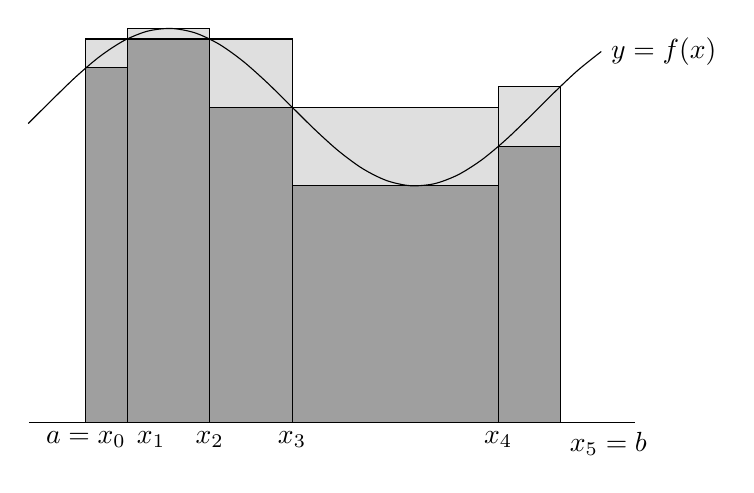
\begin{tikzpicture}
    \draw (-0.2,0)--(7.5,0);
    \filldraw[fill=lightgray!50,draw=black](pi/6,{sin(pi/6 r)+4}) rectangle (pi/3,{sin(pi/3 r)+4});
    \filldraw[fill=darkgray!50,draw=black](pi/6,0) rectangle (pi/3,{sin(pi/6 r)+4});
    \filldraw[fill=lightgray!50,draw=black](pi/3,{sin(pi/3 r)+4}) rectangle ({2*pi/3},5);
    \filldraw[fill=darkgray!50,draw=black](pi/3,0) rectangle ({2*pi/3},{sin(pi/3 r)+4});
    \filldraw[fill=lightgray!50,draw=black]({2*pi/3},{sin(pi r)+4}) rectangle (pi,{sin(2*pi/3 r)+4});
    \filldraw[fill=darkgray!50,draw=black]({2*pi/3},0) rectangle ({pi},{sin(pi r)+4});
    \filldraw[fill=lightgray!50,draw=black]({pi},3) rectangle ({11*pi/6},{sin(pi r)+4});
    \filldraw[fill=darkgray!50,draw=black]({pi},0) rectangle ({11*pi/6},3);
    \filldraw[fill=lightgray!50,draw=black]({11*pi/6},{sin(11*pi/6 r)+4}) rectangle ({25*pi/12},{sin(25*pi/12 r)+4});
    \filldraw[fill=darkgray!50,draw=black]({11*pi/6},0) rectangle ({25*pi/12},{sin(11*pi/6 r)+4});
    \draw (pi/6,0) node [below] {$a=x_0$};
    \draw (pi/3,0) node [below right] {$x_1$};
    \draw (2*pi/3,0) node [below] {$x_2$};
    \draw (pi,0) node [below] {$x_3$};
    \draw (11*pi/6,0) node [below] {$x_4$};
    \draw (25*pi/12,0) node [below right] {$x_5=b$};
    \draw [domain={-pi/15}:{27*pi/12},smooth] plot(\x, {sin(\x r) +4}) node [right]{$y=f(x)$};
  \end{tikzpicture} 
  \caption{上方和と下方和}
  \end{figure}

\deref{上方和・下方和}において，$f$は$[a,b]$で有界だから，任意の$x \in [a,b]$に対して
\[
    m \leqq f(x) \leqq M
\]
となるような$m ,M \in \mathbb{R}$が存在する．

これより，
\[
    m(b-a) \leqq L(f,P) \leqq U(f,P) \leqq M(b-a)
\]
を得て，$L(f,P)$，$U(f,P)$はともに有界であることがわかった．

\begin{definition}{細分}{細分}
	 区間$[a,b]$の分割$P^{\ast}$で，$P$の全ての分割が$P^{\ast}$の分割でもあるとき，$P^{\ast}$を$P$の細分という．
\end{definition}

\begin{prop}{細分と上方和・下方和}{細分と上方和・下方和}
	$P^{\ast}$を$P$の細分とするとき，
	\begin{align*}
		&U(f,P^{\ast})\leqq U(f,P),\\
		&L(f,P) \leqq L(f,P^{\ast})
	\end{align*}
	である．
\end{prop}

\begin{tleftbar}
	\begin{proof} 
		上方和について証明する．

		分割$P$に，$x_{i-1} \leqq x^{\ast} \leqq x_i$をみたす点$x^{\ast}$を付け加えた細分を$P^{\ast}$とする．

		このとき，$U(f,P)$と$U(f,P^{\ast})$は，前者の$M_i (x_i-x_{i-1})$の項が後者だと
		\[
			M_i ' (x^{\ast}-x_{i-1}) +M_i '' (x_i-x^{\ast})
		\]
		に変わる点のみが異なる．ただしここで$M_i ' \coloneqq \sup_{x_{i-1} \leqq x \leqq x^{\ast}} f(x)$，
		$M_i '' \coloneqq \sup_{x^\ast \leqq x \leqq  x_i} f(x)$とした．

		$M_i$，$M_i ' $，$M_i ''$の定義から
		\[
			M_i ' \leqq M_i , \quad M_i '' \leqq M_i
		\]
		なので，
		\begin{align*}
			M_i ' (x^{\ast}-x_{i-1}) +M_i '' (x_i-x^{\ast}) &\leqq M_i (x^{\ast}-x_{i-1}) + M_i(x_i -x^{\ast}) \\
			& = M_i (x_i - x_{i-1})
		\end{align*}
		となる．これよりただちに
		\[
			U(f,P^\ast) \leqq U(f,P)
		\]
		が従う．下方和についても同様である．
	\end{proof}
\end{tleftbar}
	
\begin{prop}{}{}
	有界閉区間上の連続関数は積分可能である．
\end{prop}

\begin{tleftbar}
	\begin{proof}
		$f$を$[a,b]$上で連続な関数とする．このとき，任意の$\varepsilon >0$に対して，ある$\delta >0$が存在して，任意の$x,y \in [a,b]$に対して，
		$\abs{x-y}<\delta$のとき$\abs{f(x)-f(y)}<\varepsilon$となる．

		ここで，幅が$\delta$以下の分割$P=(a_i)_{i \in \{0,1,2,\ldots,n \}}$を考える．このとき，$[a_{i-1},a_i]$の点で
		\[
			f(x_i)=m_i (f,P),\quad f(y_i)=M_i (f,P)
		\]
		なるものが存在する．

		$\abs{x_i-y_i}\leqq \delta$であるから，$f(y_i)-f(x_i)<\varepsilon$となる．よって
		\[
			U(f,P)-L(f,P) = \sum_{i=1}^{n} ( f(y_i)-f(x_i) ) (a_i-a_{i-1}) <(b-a)\varepsilon 
		\]
		となる．

		ここで，$L(f,P) \leqq L(f) \leqq U(f) \leqq U(f,P)$なので，$L(f)=U(f)$となり，$f$は積分可能である．
	\end{proof}
\end{tleftbar}
\phantomsection
\section{定積分の性質}

\begin{prop}{}{}
	$f$が連続であるならば，
	\[
		\int_{a}^{b} f(x)\, dx = \int_{a}^{c} f(x)\, dx + \int_{c}^{b} f(x)\, dx
	\]
	が成立する．
\end{prop}

証明略．

\begin{prop}{線型性}{線型性}
	連続関数$f$，$g$に対して，
	\[
		\int_{a}^{b} (kf(x)+lg(x))\, dx = k\int_{a}^{b} f(x)\, dx + l\int_{a}^{b} g(x)\, dx
	\]
	が成立する．
\end{prop}

証明略．


\begin{definition}{リーマン和}{リーマン和}
	有界閉区間$[a,b]$上の有界関数$f$に対して，$P=(x_i)_{i \in \{0,1,2,\ldots,n\}}$を分割とする．

	さらには，$\xi_i \in [x_{i-1},x_i]$を適当に選ぶ．
	
	このとき，
	\[
		\sum_{i=1}^{n} f(\xi_i)(x_i - x_{i-1})
	\]
	を分割$P$と代表点$(\xi_i)_{i \in \{1,2,\ldots,n\} }$による$f$のリーマン和といい，
	\[
		R(f,P,\xi)
	\]
	と表す．
\end{definition}


\part*{\texorpdfstring{積分($n$次元)}{積分(n次元)}}

\begin{definition}{}{}
	$n$次元の有界閉区間
	\begin{align*}
	I&=[a_1,b_1] \times [a_2,b_2] \times \cdots \times [a_n,b_n] \\
	& = \{ (x_1,x_2,\ldots,x_n) \mid a_i \leqq x_i \leqq b_i , i \in \{1,2,\dots,n \} \}
	\end{align*} 
	の$n$次元体積を，
	\[
		v(I) = \prod_{i=1}^{n} (b_i-a_i)
	\]
	と定義する．
\end{definition}

\begin{definition}{}{}
	区間$I$に対して，集合 $D(I)$を
	\[
		D(I) = \{ (x_i)_{i \in \{0,1,\ldots,n \}} \mid a=x_0 < x_1<\dots < x_n =b , n \in \mathbb{N} \}
	\]
	とする．
\end{definition}

\begin{prop}{}{}
	$D(I)$は $(a,b)$の有限部分集合全体の集合$P((a,b))$と一対一に対応する．ただし，$a=b$のときは$a$を分点とする分割を考える．
\end{prop}

\begin{tleftbar}
	\begin{proof}
		写像$f$を
		\[
			f \colon D(I) \ni (x_i)_{i \in \{0,1,\ldots,n \}} \mapsto (x_i)_{i \in \{1,\ldots,n-1 \}} \in P((a,b))
		\]
		とする．このとき，$f$が全単射であることを示す．
		\begin{description}
			\item[単射であること] まず，$(x_i)_{i \in \{0,1,\ldots,n \}} \neq (y_i)_{i \in \{0,1,\ldots,n\}}$とする． 
			このとき，ある$j \in \{0,1,\ldots,n \}$に対して，$ x_j \ne y_j $である．特に$ j \ne 0$かつ$j \ne n$のとき，
			\begin{align*} 
				& (x_i)_{i \in \{1,2,\ldots,n-1 \}} \neq (y_i)_{i \in \{1,2,\ldots,n-1\}}, \\
				& \therefore ~ f((x_i)_{i \in \{0,1,\ldots,n \}}) \neq f((y_i)_{i \in \{0,1,\ldots,n\}})
			\end{align*} 
			となるため，$f$は単射である．
			\item[全射であること] 任意の$(x_i)_{i \in \{1,\ldots,n-1 \}} \in P((a,b))$に対して，$a$および$b$を初項と末項に設定し，
			有限点列として
			\[
			(a,x_1,x_2,\ldots,x_{n-1},b)
			\]
			を考えると，これは$(x_0,x_1,\ldots,x_{n-1},x_n)$に等しい．ゆえにこのとき
			\[
			f((x_i)_{i \in \{0,1,\ldots,n\}})=(x_i)_{i \in \{1,\ldots,n-1 \}}
			\]
			となる$(x_i)_{i \in \{1,\ldots,n-1 \}} \in D(I)$が存在し，$f$は全射である．
		\end{description}
		以上の考察により，$f$は単射かつ全射，すなわち全単射である．
	\end{proof}
\end{tleftbar}

\end{comment}
\newpage  



\newpage
\phantomsection

\part*{参考文献}

\noindent
本書は\cite{sugiura}，\cite{matsuzaka}，\cite{saito}を参考にした．

\medskip

\printbibliography[heading=none]
% 索引
\clearpage
\thispagestyle{empty}
\setcounter{section}{6}
\renewcommand{\indexname}{索引}

\begingroup
  \let\section\part
  \pagestyle{empty}
  \printindex
\endgroup



% 裏表紙（表紙と同じダーク・モノトーン）
% 冊子印刷などで裏表紙を偶数ページに揃えたい場合は \MathNoteBackCover* にする
\MathNoteBackCover{Analysis}{2026 Edition}



\end{document}